\documentclass[a4paper,12pt]{book} % nie: report!

\usepackage{tikz}
\usetikzlibrary{arrows.meta,positioning}

\usepackage[T1,plmath]{polski} % lepiej to zamiast babel!

\usepackage[utf8]{inputenc} % w razie kłopotów spróbować: \usepackage[utf8x]{inputenc}
\usepackage{fancyhdr} % nagłówki i stopki
\usepackage{indentfirst} % WAŻNE, MA BYĆ!
\usepackage[pdftex]{graphicx} % to do wstawiania rysunków
\usepackage{amsfonts} % pakiety od AMS, ułatwiają składanie pewnych techniczno-matematcyznych rzeczy
\usepackage{amsmath} % to do dodatkowych symboli, przydatne
\usepackage{amssymb} % to też do dodatkowych symboli, też przydatne
\usepackage{amsthm}
\usepackage[pdftex,
            left=1.1in,right=1.1in,
            top=1.1in,bottom=1.1in]{geometry} % marginesy
\usepackage{float}
\usepackage[font=small,labelfont=bf]{caption}

\usepackage[colorlinks=true]{hyperref} % odnośniki interaktywne w PDFie
\usepackage{xurl}
\hypersetup{allcolors=black}
\usepackage{listings}
\renewcommand{\lstlistlistingname}{Spis listingów}
\lstset{
    basicstyle=\footnotesize\tt,
    numbers=left,
    numberstyle=\tiny,
    frame=tb,
    tabsize=4,
    columns=fixed,
    showstringspaces=false,
    showtabs=false,
    keepspaces,
    commentstyle=\color{red},
    keywordstyle=\color{blue}
}
\newfloat{lstfloat}{htbp}{lolst}[chapter]
\floatname{lstfloat}{Listing}
\def\lstfloatautorefname{Listing}

% jesli potrzeb, można oczywiście wstawić inne pakiety i swoje definicje...

\lstdefinelanguage{CSharp}{
  morekeywords={
    abstract, as, base, bool, break, byte, case, catch, char, checked,
    class, const, continue, decimal, default, delegate, do, double, else,
    enum, event, explicit, extern, false, finally, fixed, float, for, foreach,
    goto, if, implicit, in, int, interface, internal, is, lock, long, namespace,
    new, null, object, operator, out, override, params, private, protected,
    public, readonly, ref, return, sbyte, sealed, short, sizeof, stackalloc,
    static, string, struct, switch, this, throw, true, try, typeof, uint,
    ulong, unchecked, unsafe, ushort, using, virtual, volatile, void, while,
    var
  },
  sensitive=true,
  morecomment=[l]{//},
  morecomment=[s]{/*}{*/},
  morestring=[b]",
}

\lstset{
  basicstyle=\footnotesize\ttfamily,
  numbers=left,
  numberstyle=\tiny,
  frame=tb,
  tabsize=4,
  columns=fixed,
  showstringspaces=false,
  showtabs=false,
  keepspaces=true,
  commentstyle=\color{red!60!black},
  keywordstyle=\color{blue!70!black},
}

% definicje nagłówków i stopek
\pagestyle{fancy}
\renewcommand{\chaptermark}[1]{\markboth{#1}{}}
\renewcommand{\sectionmark}[1]{\markright{\thesection\ #1}}
\fancyhf{}
\fancyhead[LE,RO]{\footnotesize\bfseries\thepage}
\fancyhead[LO]{\footnotesize\rightmark}
\fancyhead[RE]{\footnotesize\leftmark}
\renewcommand{\headrulewidth}{0.5pt}
\renewcommand{\footrulewidth}{0pt}
\addtolength{\headheight}{1.5pt}
\fancypagestyle{plain}{\fancyhead{}\cfoot{\footnotesize\bfseries\thepage}\renewcommand{\headrulewidth}{0pt}}


% interlinia
\linespread{1.25}



\begin{document}
\begin{titlepage}
% ~

\begin{tabular}{c@{\hspace{21mm}}|@{\hspace{5mm}}l}
\vspace{-20mm} & \\
\multicolumn{2}{l}{\hspace{-12.5mm} 
\includegraphics[width=8cm]{LogoUMCS.jpg}} \\
\multicolumn{2}{@{\hspace{20mm}}l}{\vspace{-4mm}} \\
\multicolumn{2}{@{\hspace{28mm}}l}{\Large \sf UNIWERSYTET MARII
	CURIE-SKŁODOWSKIEJ} \\
\multicolumn{2}{@{\hspace{28mm}}l}{\vspace{-4mm}} \\
\multicolumn{2}{@{\hspace{28mm}}l}{\Large \sf W LUBLINIE} \\
\multicolumn{2}{@{\hspace{28mm}}l}{\vspace{-4mm}} \\
\multicolumn{2}{@{\hspace{28mm}}l}{\Large \sf Wydział Informatyki i Matematyki UMCS} \\
\multicolumn{2}{@{\hspace{28mm}}l}{\vspace{21mm}} \\
& {\sf Kierunek: \textbf{Informatyka} } \\
%& {\sf Specjalność: \textbf{informatyczna}} \\ % wpisujemy tylko jeśli jest!!!
& \\\\\\
& {\sf \large \bfseries Oleksii Burlia} \\
& \\\\\\
& \Large \sf \bfseries Algorytmy wykorzystywane w grach\\
& \Large \sf \bfseries  typu sandbox i ich implementacja\\\\[-20pt]
& \Large \sf \bfseries na platformie Unity\\\\
& {\large \sf Algorithms used in sandbox games } \\
 & {\large \sf and their implementation on the Unity platform } \\
& \\
& \\
& \\
& {\sf Praca licencjacka}  \\
& \vspace{-7mm} \\
&  {\sf napisana w Katedrze Cyberbezpieczeństwa i Lingwistyki Komputerowej} \\
&  {\sf Instytutu Informatyki UMCS} \\
& \vspace{-7mm} \\
& {\sf pod kierunkiem \bfseries dra. hab. Jarosława Byliny, prof. UMCS} \\
\multicolumn{2}{@{\hspace{28mm}}l}{\vspace{15mm}} \\
\multicolumn{2}{@{\hspace{28mm}}l}{\textbf{\textsf{Lublin 2025}}}
\end{tabular}
\end{titlepage}





\sloppy



\thispagestyle{empty}


\newpage{}

\thispagestyle{empty}

\newpage{}



\tableofcontents{}

\chapter*{Wstęp} % z gwiazdką, więc bez numerka...
\addcontentsline{toc}{chapter}{Wstęp} % ...ale w spisie treści ma być...
\chaptermark{Wstęp} % ...i w paginie górnej

Celem niniejszej pracy jest zaprojektowanie oraz implementacja prototypowej gry komputerowej gatunku \emph{sandbox} w środowisku Unity. Opracowana aplikacja ma charakter prostej „piaskownicy”, w której gracz może narysować własne obiekty, umieścić je na mapie, a następnie przeprowadzić symulację ich zachowania w interakcji z graczem i prostą sztuczną inteligencją. Szczególna uwaga została położona na algorytmy, które odgrywają kluczową rolę w implementacji.  

Pierwszy rozdział zawiera charakterystykę gier typu sandbox. Omówiona zostanie definicja tego gatunku, jego najpopularniejsze przykłady, a także zastosowanie gier sandbox w edukacji i innych dziedzinach. Na końcu przedstawiona zostanie również krytyka związana z tym typem rozgrywki.  

W drugim rozdziale zaprezentowane zostaną algorytmy wykorzystywane w grach sandboxowych. Zostanie przypomniana definicja algorytmu oraz pojęcie złożoności obliczeniowej. Następnie opisane będą algorytmy rysowania (koła i linii), ich powiązania z morfologią matematyczną oraz alternatywne rozwiązania. Kolejna część dotyczyć będzie przycinania tekstury na podstawie obwiedni, a następnie algorytmów wyszukiwania ścieżek – przede wszystkim A*, ale również innych metod oraz ich porównania. Rozdział zakończy się omówieniem maszyn stanów skończonych (FSM) wraz z przykładami stanów.  

Trzeci rozdział poświęcony jest implementacji wybranych algorytmów w Unity. Na początku zostanie przedstawione środowisko Unity i jego możliwości. Omówione zostanie także porównanie Unity z innymi silnikami gier. Następnie zaprezentowana zostanie zaimplementowana gra: jej etap edycji (rysowanie i umieszczanie obiektów) oraz etap symulacji (zachowania gracza i NPC). Kolejne podsekcje obejmują implementację metody rysowania, proces tworzenia niestandardowych koliderów, szczegółowy opis algorytmu A* w kontekście gry, a także implementację sztucznej inteligencji NPC w oparciu o maszynę stanów.  

Pracę zamyka podsumowanie, w którym przedstawione zostaną wnioski wynikające z przeprowadzonej analizy i implementacji oraz możliwe kierunki dalszego rozwoju projektu.  


\chapter{Charakterystyka gier typu sandbox}

\section{Definicja gier typu sandbox}

\textbf{Piaskownica} (ang. \texttt{sandbox}) to gatunek gier komputerowych, w których gracz może wchodzić w interakcję z elementami świata gry w niemal nieograniczony sposób \cite{Sandbox_definition}. Zazwyczaj gry tego typu nie posiadają jasno określonego celu, dlatego to gracz decyduje, jakie działania podejmie i w jakim kierunku rozwinie swoją rozgrywkę. Często wykorzystują one koncepcję otwartego świata, co zapewnia swobodę eksploracji i interakcji. Taka forma rozgrywki pozwala również na integrację z innymi gatunkami, czyniąc gry typu sandbox wyjątkowo elastycznymi pod względem projektowania.

\section{Popularne przykłady}

Jednym z najbardziej znanych i wpływowych przykładów gry typu sandbox jest \textit{Minecraft}, który od kilkunastu lat pozostaje w czołówce najpopularniejszych tytułów na świecie. Pierwsze wersje gry zostały stworzone przez szwedzkiego dewelopera Markusa Perssona („Notch”) w 2009 roku, a oficjalna premiera miała miejsce w 2011 roku \cite{Minecraft_info}. \textit{Minecraft} oferuje graczom ogromny, proceduralnie generowany świat, możliwość eksploracji, budowy, rzemiosła i przetrwania. Charakteryzuje się unikatową, pikselową grafiką oraz szerokim zakresem możliwości twórczych.

\begin{figure}[htbp]
    \centering
    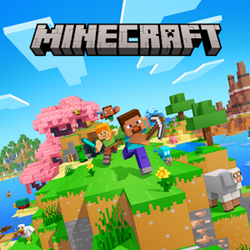
\includegraphics[width=0.6\textwidth]{images/minecraft.png}
    \caption{Przykładowy widok z gry \textit{Minecraft} \cite{Minecraft_image}.}
    \label{fig:algorytm}
\end{figure}

Innym znanym przykładem jest \textit{SimCity}, zapoczątkowane w 1989 roku przez Willa Wrighta \cite{Simcity_info}. Gra polega na swobodnym budowaniu i zarządzaniu miastem --- jego infrastrukturą, ekonomią, polityką i kulturą. Dzięki różnorodnym strategiom rozgrywki każda kampania może wyglądać inaczej. Popularność tej serii przyczyniła się również do powstania \textit{The Sims}, które rozwinęło ideę symulacji codziennego życia i również zawiera wiele cech typowych dla sandboxów.

\begin{figure}[htbp]
    \centering
    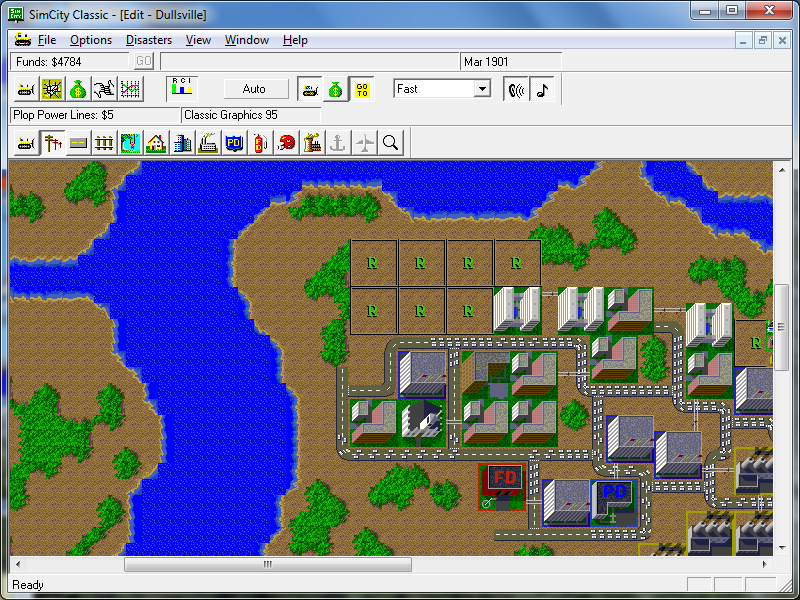
\includegraphics[width=0.8\textwidth]{images/simcity.png}
    \caption{Przykładowy widok z gry \textit{Simcity} \cite{Simcity_image}.}
    \label{fig:algorytm}
\end{figure}

Nowocześniejszym przykładem jest \textit{Don't Starve}, wydane w 2013 roku przez Klei Entertainment. Gracz wciela się w naukowca Wilsona, który trafia do tajemniczego, niebezpiecznego świata. Chociaż gra jest przede wszystkim tytułem z gatunku survival, twórcy zainspirowani sukcesem \textit{Minecrafta} wprowadzili elementy sandboxowe, takie jak otwartość świata i swoboda eksploracji, co znacząco wzbogaciło doświadczenie rozgrywki.

\begin{figure}[htbp]
    \centering
    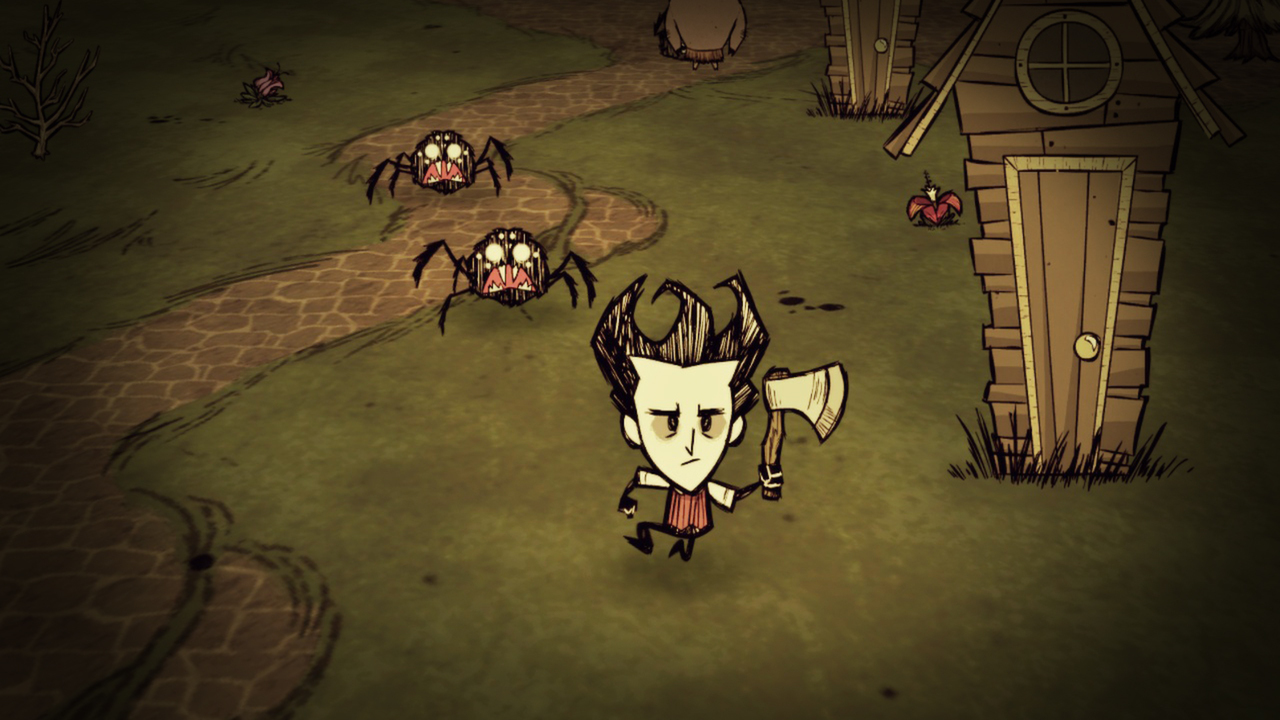
\includegraphics[width=0.8\textwidth]{images/dontstarve.jpg}
    \caption{Przykładowy widok z gry \textit{Don't Starve} \cite{Dontstarve_image}.}
    \label{fig:algorytm}
\end{figure}

\section{Zastosowanie gier sandbox w edukacji i innych dziedzinach}

Gry typu sandbox są nie tylko źródłem rozrywki, ale coraz częściej znajdują zastosowanie w edukacji, symulacjach i rozwoju umiejętności. Ich otwarta struktura sprzyja kreatywnemu myśleniu, eksperymentowaniu oraz nauce poprzez zabawę.

Przykładem może być \textit{Minecraft}, który oprócz trybu rozgrywki nastawionego na przetrwanie, zawiera wiele elementów edukacyjnych. Gracz uczy się zdobywania pożywienia, budowy schronienia, przetwarzania surowców czy tworzenia narzędzi. Proces wytwarzania (craftingu) opiera się na logicznych schematach, które rozwijają pamięć i uczą podstawowych zasad przetwarzania materiałów --- np. szkło powstaje z piasku, a węgiel drzewny z drewna. Wersja edukacyjna \textit{Minecraft Education Edition} oferuje dodatkowe materiały dydaktyczne dla nauczycieli, wspierając rozwój kompetencji uczniów w ciekawy i angażujący sposób \cite{Minecraft_education}.

Innym przykładem jest  \textit{Sandbox – Physics Simulator}, który pozwala na eksperymentowanie z reakcjami fizycznymi i chemicznymi. Gracz może obserwować, jak różne substancje oddziałują ze sobą – np. woda paruje pod wpływem ognia, śnieg topnieje, drewno się pali i przekształca w węgiel drzewny, a proch eksploduje.

Z kolei seria \textit{The Sims} pełni funkcję symulacji życia codziennego. Gracze podejmują decyzje dotyczące pracy, budżetu, relacji międzyludzkich czy budowy domu. Dzięki temu młodsze osoby mogą w przystępny sposób poznać podstawy zarządzania finansami i rozumieć konsekwencje codziennych decyzji.

\section{Krytyka}

Mimo licznych zalet, gry typu sandbox są również przedmiotem krytyki. Ze względu na brak jasno określonych celów i dużą swobodę, niektórzy gracze postrzegają je jako niedopracowane lub mało angażujące. Twórca gier komputerowych, Ernest Adams, zauważył:
\begin{quote}
„Wrzucenie gracza do piaskownicy i powiedzenie mu ‘baw się dobrze’ nie wystarczy. Zwłaszcza na początku gry gracz powinien mieć jasne poczucie tego, co robi dalej, a w szczególności --- dlaczego.” \cite{Quote_1}.

\end{quote}

Podobną opinię wyraził Christopher Totten:
\begin{quote}
„Elementy piaskownicy mogą być błędnie traktowane jako uczciwy zamiennik treści narracyjnych; w rzeczywistości wiele gier zaprzepaściło swój potencjał, ponieważ wyobrażały sobie, że swobodna rozgrywka zrekompensuje brak narracji. Ale nawet dla naszego wyidealizowanego dziecka zabawa w fizycznej piaskownicy szybko się nudzi.” \cite{Quote_2}.
\end{quote}

Krytycy podkreślają, że:
\begin{quote}
„Wielkim ryzykiem piaskownicy jest to, że może być nudna. Dzieje się tak, ponieważ sam ‘piasek’ nie daje zbyt wiele frajdy. Zautomatyzowana, złożona i – być może przede wszystkim – ukierunkowana responsywność jest niezbędna do zabawy w piaskownicy. Im bardziej złożony i interaktywny świat, tym bardziej interesująca staje się rozgrywka.” \cite{Quote_3}.
\end{quote}

Tego typu krytyka jest uzasadniona – zbyt proste mechanizmy bez dodatkowego kontekstu fabularnego mogą szybko prowadzić do znudzenia. Dlatego coraz częściej łączy się elementy piaskownicy z innymi gatunkami, takimi jak RPG, survival czy strategie, aby stworzyć bardziej angażujące doświadczenia.

\chapter{Algorytmy używane w grach typu sandbox}
W tej części pracy omówione zostaną wybrane algorytmy, które odgrywają istotną rolę w tworzeniu gier typu \textit{sandbox}. Skupimy się zarówno na ich definicjach teoretycznych, jak i na sposobach praktycznej implementacji. Przedstawione metody obejmują m.in. algorytmy rysowania, przeszukiwania ścieżki, tworzenia niestandardowych brył kolizyjnych, a także mechanizmy związane z obsługą fizyki w środowisku gry.

Warto zaznaczyć, że omawiane rozwiązania bazują na algorytmach, które autor niniejszej pracy samodzielnie zaimplementował w stworzonym przez siebie projekcie gry. Dzięki temu możliwe jest zaprezentowanie zarówno teoretycznych podstaw, jak i praktycznych aspektów implementacji, popartych przykładami kodu źródłowego.

\section{Definicja algorytmu}

\textbf{Algorytm} można zdefiniować jako skończony, uporządkowany zbiór jasno określonych instrukcji, których wykonanie prowadzi do rozwiązania danego problemu lub osiągnięcia określonego celu \cite{Algorithms_introduction}. Instrukcje te muszą być wykonalne w skończonym czasie oraz zrozumiałe dla wykonawcy — zarówno człowieka, jak i maszyny.

W kontekście informatyki i programowania algorytm rozumiemy jako precyzyjny opis procedury obliczeniowej realizowanej przez komputer.
Innymi słowami, algorytm to każdy jednoznacznie określony proces obliczeniowy, który przyjmuje pewną wartość lub zbiór wartości jako dane wejściowe, a następnie generuje określoną wartość lub zbiór wartości jako wynik. Algorytm można zatem postrzegać jako sekwencję kroków obliczeniowych, które przekształcają dane wejściowe w dane wyjściowe.
Można go również traktować jako narzędzie do rozwiązywania ściśle zdefiniowanego problemu obliczeniowego. Opis problemu w ogólnych kategoriach określa pożądany związek pomiędzy danymi wejściowymi a wynikami, natomiast algorytm precyzuje konkretną procedurę obliczeniową, która ten związek realizuje.

\subsection*{Przykłady intuicyjne}

Aby lepiej zrozumieć istotę algorytmu, można posłużyć się prostymi przykładami:

\begin{itemize}
    \item \textbf{Algorytm rysowania koła:} dane wejściowe to współrzędne środka i promień $r$, a wynikiem jest zbiór pikseli, które należy zamalować, aby na ekranie pojawiło się koło.
    \item \textbf{Algorytm wyszukiwania ścieżki:} dane wejściowe to mapa gry i pozycje dwóch punktów, a wynikiem jest najkrótsza sekwencja kroków prowadzących od punktu startowego do celu.
    \item \textbf{Algorytm detekcji kolizji:} dane wejściowe to pozycje i rozmiary obiektów, a wynikiem jest informacja, czy dane obiekty nachodzą na siebie, czy też nie.
\end{itemize}

We wszystkich tych przykładach można wyróżnić trzy elementy:
\begin{enumerate}
    \item \textbf{Dane wejściowe (Input):} informacje przekazywane algorytmowi, np. współrzędne, mapa czy zestaw obiektów.
    \item \textbf{Zestaw instrukcji (Procedura):} skończony, uporządkowany opis kroków do wykonania.
    \item \textbf{Dane wyjściowe (Output):} wynik działania, np. narysowany obiekt, ścieżka lub informacja o kolizji.
\end{enumerate}

Dzięki temu algorytm można porównać do przepisu kulinarnego: składniki to dane wejściowe, sposób przygotowania to procedura, a gotowe danie to wynik.

\subsection{Złożoność obliczeniowa algorytmów}

Efektywność algorytmu mierzy się często za pomocą jego \emph{złożoności obliczeniowej}, czyli liczby podstawowych operacji wykonanych w zależności od wielkości danych wejściowych. W praktyce najważniejsza jest analiza zachowania algorytmu w granicach dużych danych, co umożliwia porównanie różnych metod niezależnie od konkretnego sprzętu.

Do opisu tempa wzrostu złożoności obliczeniowej zwykle wykorzystuje się tzw. \emph{notację wielkiego O} (ang. \texttt{Big O notation}) \cite{Algorithms_introduction}. Jest to matematyczny sposób określania górnej granicy wzrostu funkcji opisującej liczbę operacji wykonywanych przez algorytm w zależności od wielkości danych wejściowych. Dzięki temu możliwe jest sklasyfikowanie algorytmów według ich efektywności oraz porównywanie ich niezależnie od implementacji czy parametrów technicznych komputera.

\subsection*{Intuicja notacji \(O(n)\)}

Notacja \(O(n)\) nie podaje dokładnej liczby operacji, ale określa \textbf{jak szybko} rośnie czas działania algorytmu wraz ze wzrostem rozmiaru danych wejściowych. Na przykład:
\begin{itemize}
    \item algorytm o złożoności \(O(1)\) (\textit{czas stały}) — wykonuje tę samą liczbę operacji niezależnie od liczby danych (np. odczyt elementu tablicy po indeksie),
    \item algorytm o złożoności \(O(n)\) (\textit{czas liniowy}) — czas działania rośnie proporcjonalnie do liczby elementów (np. zsumowanie wszystkich elementów tablicy),
    \item algorytm o złożoności \(O(n^2)\) (\textit{czas kwadratowy}) — liczba operacji rośnie proporcjonalnie do kwadratu liczby danych (np. sortowanie bąbelkowe),
    \item algorytm o złożoności \(O(\log n)\) (\textit{czas logarytmiczny}) — bardzo wydajny, ponieważ nawet dla dużych danych liczba operacji rośnie powoli (np. wyszukiwanie binarne).
\end{itemize}

Formalnie, zbiór funkcji należących do notacji \(O(g(n))\) można zdefiniować w następujący sposób:
\[
O(g) = \left\{ f : \exists c>0,\,\exists n_0,\ \forall n \ge n_0,\; 0 \le f(n) \le c\,g(n) \right\}.
\]

\subsection*{Złożoność czasowa}

Najczęściej analizowaną miarą jest \textbf{złożoność czasowa} (ang. \textit{time complexity}), czyli przybliżona liczba kroków, jakie algorytm musi wykonać w zależności od danych wejściowych. Analiza ta nie mówi, ile milisekund zajmie program, ale pozwala porównać, czy jeden algorytm rośnie szybciej czy wolniej od drugiego przy dużych danych. 

Na przykład, algorytm liniowy \(O(n)\) dla tablicy o rozmiarze \(10^6\) wykona około miliona operacji, podczas gdy algorytm kwadratowy \(O(n^2)\) dla tej samej tablicy — aż trylion (\(10^{12}\)) operacji, co czyni go w praktyce nieużytecznym dla tak dużych danych.

\subsection*{Złożoność pamięciowa}

Drugim istotnym aspektem jest \textbf{złożoność pamięciowa} (ang. \textit{space complexity}), która określa, jak dużo dodatkowej pamięci (RAM) potrzebuje algorytm podczas działania. 

Przykłady:
\begin{itemize}
    \item algorytm o złożoności pamięciowej \(O(1)\) wymaga stałej ilości pamięci, niezależnej od wielkości danych (np. proste zliczanie elementów w tablicy),
    \item algorytm o złożoności \(O(n)\) potrzebuje dodatkowej pamięci proporcjonalnej do liczby danych wejściowych (np. kopiowanie tablicy),
    \item bardziej złożone struktury, takie jak algorytmy grafowe, mogą wymagać pamięci \(O(n^2)\), jeśli muszą przechowywać pełną macierz sąsiedztwa dla grafu z \(n\) wierzchołkami.
\end{itemize}

Analiza pamięciowa jest szczególnie ważna w systemach o ograniczonych zasobach, takich jak urządzenia mobilne czy wbudowane.

\section{Algorytmy rysowania}

Funkcja rysowania w omawianej grze składa się z dwóch podstawowych elementów:
\begin{itemize}
    \item rysowania wypełnionego koła w miejscu kliknięcia kursora,
    \item łączenia kolejnych kół wzdłuż trajektorii kursora w celu uzyskania linii ciągłej.
\end{itemize}

Każdy z tych kroków można opisać osobnym algorytmem, a ich połączenie daje mechanizm działania pędzla.

\subsection{Algorytm rysowania koła}

Podstawowym podejściem zastosowanym w grze jest \textbf{rasteryzacja koła}  \cite{Rasteryzacja} oparta na równaniu matematycznym:
\[
x^2 + y^2 \leq r^2
\]
Dla każdego piksela $(x,y)$ sprawdzane jest, czy spełnia warunek przynależności do wnętrza koła o promieniu $r$. 
Jeżeli tak, piksel zostaje zamalowany wybranym kolorem. 
Jest to przykład procesu rasteryzacji, czyli zamiany figury opisanej matematycznie na zbiór dyskretnych punktów (pikseli) na ekranie.

\begin{lstlisting}[language=C++, caption={Przykład algorytmu rysowania koła}, label={lst:circle}]
for (int i = -r; i < r; i++) {
    for (int j = -r; j < r; j++) {
        if (i*i + j*j <= r*r) {
            setPixel(x+i, y+j);
        }
    }
}
\end{lstlisting}


\subsection{Algorytm rysowania linii}

Rysowanie linii polega na \textbf{interpolacji} \cite{Interpolacja} pomiędzy kolejnymi punktami. 
Obliczany jest wektor kierunkowy od punktu początkowego do końcowego oraz dystans pomiędzy nimi. 
Następnie w równych odstępach (określonych przez wartość przesunięcia) 
wyznaczane są punkty pośrednie, w których rysowane jest koło reprezentujące pędzel. 
Tego typu podejście wykorzystuje interpolację, czyli wyznaczanie wartości pośrednich na podstawie znanych punktów.


\begin{lstlisting}[language=C++, caption={Przykład algorytmu rysowania linii}, label={lst:line}]
float distance = length(end - start);
Vector2 direction = normalize(end - start);

for (float i = 0; i < distance; i += offset) {
    Vector2 pos = start + direction * i;
    drawCircle(pos.x, pos.y, r);
}
\end{lstlisting}


\subsection{Związek z morfologią matematyczną}

Opisana metoda rysowania może być formalnie powiązana z \textbf{morfologią matematyczną} \cite{Morfologia_1, Morfologia_2}, działem przetwarzania obrazów opartym na teorii zbiorów. 
Operacja rysowania koła w punkcie kliknięcia jest w rzeczywistości przykładem \textbf{dylatacji}: pojedynczy punkt (zbiór $X$) powiększany jest o element strukturalny (zbiór $B$), którym w tym przypadku jest koło:
\[
X \oplus B = \{ x + b : x \in X, b \in B \}.
\]

Każde kliknięcie myszą można więc interpretować jako dylatację punktu przez element strukturalny w kształcie koła. 
Z kolei rysowanie linii polega na powtarzaniu tej operacji wzdłuż trajektorii ruchu kursora, co odpowiada iterowanej dylatacji zbioru punktów. 
Dzięki temu algorytm pędzla można traktować jako praktyczne zastosowanie pojęć morfologii matematycznej w kontekście grafiki komputerowej.

\subsection{Alternatywne algorytmy rysowania i porównanie}

W praktyce istnieje wiele podejść do rysowania podstawowych figur, takich jak linie czy okręgi. 
Algorytmy użyte w opisywanej grze bazują na prostych zasadach matematycznych: rasteryzacji koła na podstawie równania 
\[
x^2 + y^2 \leq r^2
\]
oraz interpolacji punktów na odcinku przy pomocy dystansu i wektora kierunkowego. 
Są one intuicyjne, łatwe do implementacji i dobrze sprawdzają się w przypadku rysowania z użyciem pędzla w aplikacji sandboxowej. 

\subsubsection*{Algorytm Bresenhama}
Jednym z najbardziej znanych i klasycznych algorytmów rysowania linii jest \textbf{algorytm Bresenhama} \cite{Bresenham}. 
Jego główną zaletą jest wydajność: do wyznaczania kolejnych pikseli wykorzystuje wyłącznie operacje całkowitoliczbowe, co czyni go bardzo szybkim. 
Algorytm ten jednak rysuje linie o grubości jednego piksela, co w przypadku narzędzia przypominającego pędzel byłoby niewystarczające. 

\subsubsection*{Algorytm Midpoint Circle}
Dla okręgów istnieje analogiczny algorytm – \textbf{algorytm rysowania okręgu metodą punktu środkowego} (ang. \texttt{Midpoint Circle Algorithm}) \cite{Midpoint_circle}. 
Podobnie jak Bresenham, wykorzystuje on tylko operacje na liczbach całkowitych i dzięki symetrii oblicza jedynie część punktów, które następnie są lustrzane w ośmiu oktantach okręgu. 
Jest to rozwiązanie szybsze niż bezpośrednie sprawdzanie równania okręgu dla każdego piksela, ale również ogranicza się do obwodu okręgu.

\subsubsection*{Porównanie}
Algorytmy klasyczne, takie jak Bresenhama czy Midpoint Circle, były projektowane z myślą o maksymalnej wydajności w czasach, gdy moc obliczeniowa komputerów była bardzo ograniczona. 
Oba algorytmy doskonale sprawdzają się w grafice niskopoziomowej (np. w systemach osadzonych czy starych bibliotekach graficznych). 
Zastosowana w grze metoda rasteryzacji koła i interpolacji linii jest jednak lepiej dostosowana do współczesnych potrzeb:
\begin{itemize}
    \item umożliwia łatwe rysowanie linii o dowolnej grubości,
    \item pozwala używać pędzla w postaci koła (a nie tylko pojedynczych pikseli),
    \item jest prostsza do rozszerzenia o inne kształty i efekty (np. gradient, przezroczystość).
\end{itemize}

Z tego względu wybór prostego algorytmu matematycznego, zamiast klasycznych metod optymalizacji, jest uzasadniony – w kontekście gry typu sandbox 
ważniejsza jest elastyczność i możliwość rozszerzania, a nie ekstremalna optymalizacja pojedynczej operacji.

\section{Przycinanie tekstury na podstawie obwiedni}

Po zakończeniu rysowania pędzlem warto zredukować rozmiar powstałej tekstury do minimalnego prostokąta, który zawiera wszystkie nieprzezroczyste piksele. Tę operację nazywamy \textbf{wyznaczeniem prostokątnej obwiedni} (ang.\ \texttt{axis-aligned bounding box, AABB}) oraz \textbf{przycinaniem obrazu} (ang.\ \texttt{image cropping}). W ujęciu przetwarzania obrazów odpowiada to wyznaczeniu obszaru zainteresowania (ROI) na podstawie binarnej maski obiektu \cite{Morfologia_1, Graphics}.

\subsection{Model i definicje}

W grafice komputerowej obrazy najczęściej reprezentuje się w modelu \textbf{RGBA} (ang. \texttt{Red, Green, Blue, Alpha}). 
Każdy piksel opisany jest czterema wartościami:
\[
(R,\,G,\,B,\,A),
\]
gdzie \(R,G,B\) oznaczają intensywności trzech barw podstawowych (czerwonej, zielonej i niebieskiej), 
a \(A\) (\emph{Alpha}) określa przezroczystość piksela w przedziale \([0,1]\) (lub w praktyce \([0,255]\) w reprezentacji całkowitoliczbowej). 
Dzięki kanałowi alfa możliwe jest odróżnienie tła od obiektu rysowanego.

Niech \(I\colon \{0,\ldots,W-1\}\times\{0,\ldots,H-1\}\to \mathbb{R}^4\) będzie obrazem RGBA o szerokości \(W\) i wysokości \(H\).
Definiujemy zbiór pikseli należących do narysowanego obiektu poprzez próg na kanale alfa:
\[
S \;=\; \{\, (x,y)\in [0,W\!-\!1]\times[0,H\!-\!1] : \alpha(x,y) \ge \tau \,\},
\]
gdzie \(\tau\in[0,1]\) jest progiem przezroczystości.

Jeżeli \(S\neq\varnothing\), minimalna \emph{obwiednia prostokątna} wyrównana do osi ma współrzędne:
\[
x_{\min}=\min_{(x,y)\in S} x,\quad
x_{\max}=\max_{(x,y)\in S} x,\quad
y_{\min}=\min_{(x,y)\in S} y,\quad
y_{\max}=\max_{(x,y)\in S} y,
\]
a jej rozmiar:
\[
\text{width}=x_{\max}-x_{\min}+1,\qquad
\text{height}=y_{\max}-y_{\min}+1.
\]

Przycięta tekstura \(I_{\text{crop}}\) jest kopią podobrazu:
\[
I_{\text{crop}}(u,v)=I(x_{\min}+u,\; y_{\min}+v),\quad
u\in[0,\text{width}-1],\; v\in[0,\text{height}-1].
\]

\begin{lstlisting}[language=C++, caption={Przykład wyznaczania prostokątnej obwiedni i przycinania (cropping)}, label={lst:crop_bbox}]
struct RGBA { uint8_t r,g,b,a; };

struct BBox { int xMin, yMin, xMax, yMax; bool valid; };

BBox computeBoundingBox(const RGBA* pixels, 
int W, int H, uint8_t alphaThreshold=1) {
    int xMin = W, xMax = -1, yMin = H, yMax = -1;
    for (int y = 0; y < H; ++y) {
        for (int x = 0; x < W; ++x) {
            const RGBA& p = pixels[y*W + x];
            if (p.a >= alphaThreshold) {
                if (x < xMin) xMin = x;
                if (x > xMax) xMax = x;
                if (y < yMin) yMin = y;
                if (y > yMax) yMax = y;
            }
        }
    }
    if (xMax < xMin || yMax < yMin) 
        return {0,0,0,0,false}; // brak nieprzezroczystych pikseli
    return {xMin, yMin, xMax, yMax, true};
}

std::vector<RGBA> cropImage(const RGBA* pixels,
int W, int H, const BBox& b, int& outW, int& outH) {
    outW = b.xMax - b.xMin + 1;
    outH = b.yMax - b.yMin + 1;
    std::vector<RGBA> cropped(outW * outH);
    for (int v = 0; v < outH; ++v) {
        for (int u = 0; u < outW; ++u) {
            cropped[v*outW + u] = pixels[(b.yMin + v)*W +
            (b.xMin + u)];
        }
    }
    return cropped;
}
\end{lstlisting}

\subsection*{Złożoność obliczeniowa}
Przejście po wszystkich pikselach to \(O(W\cdot H)\) czasu i \(O(1)\) pamięci pomocniczej; kopiowanie wycinka to \(O(\text{width}\cdot \text{height})\).
Łącznie złożoność pozostaje liniowa względem liczby pikseli obrazu wejściowego.

\section{Algorytmy przeszukiwania ścieżki}

Problem znajdowania najkrótszej ścieżki jest jednym z kluczowych zagadnień informatyki teoretycznej i praktycznej, 
szczególnie w dziedzinach takich jak sztuczna inteligencja, sieci komputerowe czy gry komputerowe.
Polega on na wyznaczeniu optymalnej trasy pomiędzy dwoma punktami (wierzchołkami) w taki sposób, aby minimalizować koszt podróży.

Formalnym modelem tego problemu jest \textbf{graf} $G = (V, E)$, gdzie $V$ oznacza zbiór wierzchołków (ang. \textit{vertices}), 
a $E$ zbiór krawędzi (ang. \textit{edges}) \cite{Algorithms_introduction}. 
Każda krawędź $(u,v) \in E$ może mieć przypisaną wagę $w(u,v)$, reprezentującą koszt przejścia między wierzchołkami $u$ i $v$. 
Zadanie algorytmu polega na znalezieniu ścieżki 
\[
P = \langle v_1, v_2, \dots, v_k \rangle
\]
łączącej punkt początkowy $s$ z punktem końcowym $t$, tak aby minimalizować sumę wag:
\[
\text{koszt}(P) = \sum_{i=1}^{k-1} w(v_i, v_{i+1}).
\]

\begin{figure}[H]
    \centering
    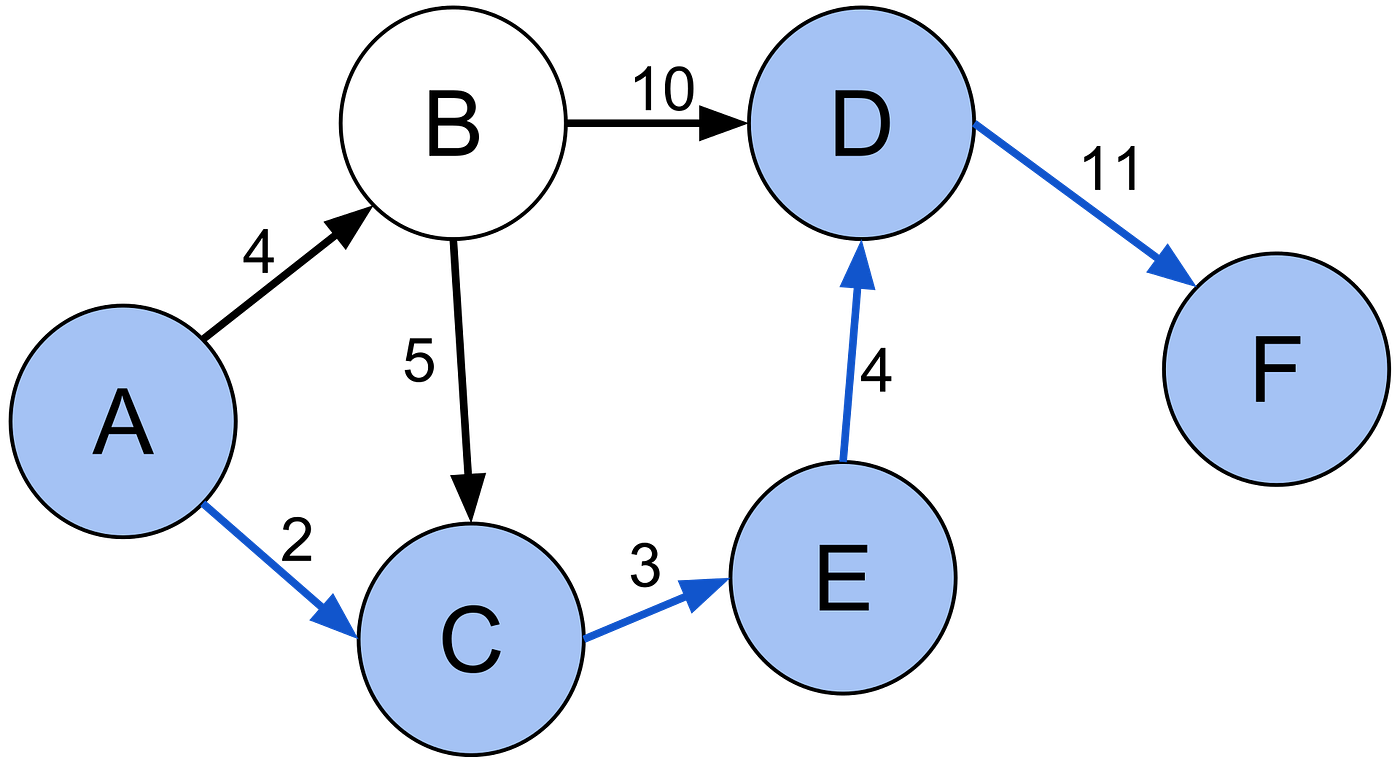
\includegraphics[width=0.55\linewidth]{images/graph.png}
    \caption{Przykładowy graf z zaznaczoną najkrótszą ścieżką pomiędzy dwoma wierzchołkami \cite{Graph_image}.}
    \label{fig:graph_example}
\end{figure}

\subsection{Algorytm A*}

Algorytm \textbf{A*} (ang. \textit{A-star}) jest jednym z najbardziej efektywnych i najczęściej stosowanych algorytmów znajdowania najkrótszej ścieżki, 
szczególnie w grach komputerowych i systemach nawigacyjnych \cite{AI}. 
Łączy on podejście dokładne (analizowanie kosztów przejścia) z podejściem heurystycznym (szacowanie odległości do celu).

\subsubsection*{Idea działania}

Algorytm A* przypisuje każdemu wierzchołkowi $n$ funkcję oceny $f(n)$:
\[
f(n) = g(n) + h(n),
\]
gdzie:
\begin{itemize}
    \item $g(n)$ – koszt dotarcia od wierzchołka początkowego $s$ do $n$,
    \item $h(n)$ – funkcja heurystyczna szacująca koszt dotarcia z $n$ do celu $t$,
    \item $f(n)$ – łączny koszt, na podstawie którego podejmowana jest decyzja o dalszej eksploracji.
\end{itemize}

W praktyce najczęściej stosuje się heurystykę opartą na odległości:
\[
h(n) = 
\begin{cases}
|x_n - x_t| + |y_n - y_t| & \text{(odległość Manhattan)},\\
\sqrt{(x_n - x_t)^2 + (y_n - y_t)^2} & \text{(odległość euklidesowa)},
\end{cases}
\]
które zapewniają dobrą równowagę pomiędzy szybkością działania a poprawnością wyników.

\subsubsection*{Kolejka priorytetowa}

Podstawowym elementem implementacji A* jest \textbf{kolejka priorytetowa} (ang. \textit{priority queue}), 
która przechowuje otwarte wierzchołki uporządkowane według wartości $f(n)$. 
Dzięki temu algorytm zawsze wybiera w pierwszej kolejności wierzchołek najbardziej obiecujący.

\begin{lstlisting}[language=C++, caption={Przykład algorytmu A*}, label={lst:astar}]
struct Node {
    int x, y;
    float g, h, f;
    Node* parent;
};

vector<Node*> AStar(Node* start, Node* goal) {
    priority_queue<pair<float, Node*>, vector<pair<float, Node*>>,
    greater<>> openSet;
    unordered_map<Node*, float> gScore;
    unordered_map<Node*, Node*> parent;

    gScore[start] = 0.0f;
    openSet.push({heuristic(start, goal), start});

    while (!openSet.empty()) {
        Node* current = openSet.top().second;
        openSet.pop();

        if (current == goal) {
            return reconstructPath(parent, goal);
        }

        for (Node* neighbor : neighbors(current)) {
            float tentative_g = gScore[current] + 
            weight(current, neighbor);

            if (!gScore.count(neighbor) || 
            tentative_g < gScore[neighbor]) {
                parent[neighbor] = current;
                gScore[neighbor] = tentative_g;
                float f = tentative_g + heuristic(neighbor, goal);
                openSet.push({f, neighbor});
            }
        }
    }

    return {};
}

\end{lstlisting}

\subsubsection*{Złożoność obliczeniowa}

Złożoność obliczeniowa A* zależy od heurystyki oraz struktury grafu.  
W najgorszym przypadku wynosi:
\[
O(E \log V),
\]
gdzie $V$ to liczba wierzchołków, a $E$ liczba krawędzi.  
W praktyce jednak, dzięki dobrej heurystyce, A* działa znacznie szybciej i eksploruje tylko część grafu.

\subsection{Inne algorytmy przeszukiwania ścieżki}

Oprócz algorytmu A*, w literaturze i praktyce stosuje się również szereg innych metod przeszukiwania grafów. 
Każdy z nich różni się założeniami, sposobem działania i złożonością obliczeniową, co sprawia, że znajdują zastosowanie w różnych kontekstach.
W poniższej części omówione zostaną najważniejsze algorytmy: BFS, DFS, Dijkstry oraz Greedy Best-First Search.

\subsubsection*{Algorytm BFS (Breadth-First Search)}
Algorytm \textbf{BFS} (\textit{przeszukiwanie wszerz}) służy do znajdowania najkrótszej ścieżki w grafach nieważonych \cite{Algorithms_introduction}. 
Działa poprzez równoległe rozszerzanie wszystkich sąsiadów danego wierzchołka, dzięki czemu zawsze znajduje ścieżkę o minimalnej liczbie kroków. Złożoność czasowa wynosi \(O(V + E)\).
W praktyce BFS jest szeroko wykorzystywany np. w labiryntach i prostych grach, gdzie wszystkie ruchy mają ten sam koszt. 

\begin{lstlisting}[language=C++, caption={Przykład algorytmu BFS}, label={lst:bfs}]
vector<Node*> BFS(Node* start, Node* goal) {
    queue<Node*> q;
    unordered_map<Node*, Node*> parent;
    unordered_set<Node*> visited;

    q.push(start);
    visited.insert(start);

    while (!q.empty()) {
        Node* current = q.front(); q.pop();
        if (current == goal) return reconstructPath(parent, goal);

        for (Node* neighbor : neighbors(current)) {
            if (!visited.count(neighbor)) {
                visited.insert(neighbor);
                parent[neighbor] = current;
                q.push(neighbor);
            }
        }
    }
    return {};
}
\end{lstlisting}

\subsubsection*{Algorytm DFS (Depth-First Search)}
Algorytm DFS (\textit{przeszukiwanie w głąb}) polega na eksploracji grafu tak daleko, jak to możliwe, zanim nastąpi powrót do poprzedniego wierzchołka \cite{Algorithms_introduction}. 
Choć nie gwarantuje znalezienia najkrótszej ścieżki, jest niezwykle prosty w implementacji i przydatny do sprawdzania spójności grafu czy wyszukiwania cykli. Złożoność czasowa wynosi \(O(V + E)\).

\begin{lstlisting}[language=C++, caption={Przykład algorytmu DFS}, label={lst:dfs}]
bool DFS(Node* start, Node* goal) {
    stack<Node*> s;
    unordered_set<Node*> visited;

    s.push(start);

    while (!s.empty()) {
        Node* current = s.top(); s.pop();
        if (current == goal) return true;

        if (!visited.count(current)) {
            visited.insert(current);
            for (Node* neighbor : neighbors(current)) {
                s.push(neighbor);
            }
        }
    }
    return false;
}
\end{lstlisting}

\subsubsection*{Algorytm Dijkstry}
Algorytm Dijkstry znajduje najkrótszą ścieżkę w grafie o nieujemnych wagach krawędzi \cite{Algorithms_introduction}. 
Działa w sposób zachłanny, wybierając w każdym kroku wierzchołek o najmniejszym koszcie dojścia i aktualizując odległości do sąsiadów. Przy użyciu \textit{priority\_queue} złożoność czasowa wynosi \(O((V + E)\log V)\).
Jest fundamentalnym algorytmem w teorii grafów i stanowi punkt odniesienia dla metod heurystycznych, takich jak A*.

\begin{lstlisting}[language=C++, caption={Przykład algorytmu Dijkstry}, label={lst:dijkstra}]
vector<Node*> Dijkstra(Node* start, Node* goal) {
    priority_queue<pair<float, Node*>, 
    vector<pair<float, Node*>>, greater<>> pq;
    unordered_map<Node*, float> dist;
    unordered_map<Node*, Node*> parent;

    for (Node* node : Graph) dist[node] = INFINITY;
    dist[start] = 0;
    pq.push({0, start});

    while (!pq.empty()) {
        Node* current = pq.top().second; pq.pop();
        if (current == goal) return reconstructPath(parent, goal);

        for (Node* neighbor : neighbors(current)) {
            float alt = dist[current] + weight(current, neighbor);
            if (alt < dist[neighbor]) {
                dist[neighbor] = alt;
                parent[neighbor] = current;
                pq.push({alt, neighbor});
            }
        }
    }
    return {};
}
\end{lstlisting}

\subsubsection*{Algorytm Greedy Best-First Search}
Algorytm Greedy Best-First Search działa podobnie do A*, ale uwzględnia wyłącznie heurystykę \(h(n)\), ignorując koszt dotarcia do wierzchołka (\(g(n)\)) \cite{AI}. 
Dzięki temu potrafi bardzo szybko znaleźć rozwiązanie, lecz nie gwarantuje optymalności. 
Stosowany jest w sytuacjach, gdzie ważna jest szybkość odpowiedzi, a nie dokładność, np. w grach komputerowych przy eksploracji dużych map. Z kolejką priorytetową złożoność czasowa wynosi \(O(E \log V)\).

\begin{lstlisting}[language=C++, caption={Przykład algorytmu Greedy Best-First Search}, label={lst:greedy}]
vector<Node*> Greedy(Node* start, Node* goal) {
    priority_queue<pair<float, Node*>, vector<pair<float, Node*>>, 
    greater<>> pq;
    unordered_set<Node*> visited;
    unordered_map<Node*, Node*> parent;

    pq.push({heuristic(start, goal), start});

    while (!pq.empty()) {
        Node* current = pq.top().second; pq.pop();
        if (current == goal) return reconstructPath(parent, goal);

        visited.insert(current);
        for (Node* neighbor : neighbors(current)) {
            if (!visited.count(neighbor)) {
                parent[neighbor] = current;
                pq.push({heuristic(neighbor, goal), neighbor});
            }
        }
    }
    return {};
}
\end{lstlisting}

\subsection{Alternatywne algorytmy przeszukiwania ścieżki i porównanie}

Przedstawione algorytmy różnią się zarówno pod względem złożoności obliczeniowej, 
jak i jakości otrzymywanych wyników. 
\begin{itemize}
    \item \textbf{BFS (Breadth-First Search)} gwarantuje znalezienie najkrótszej ścieżki, 
    ale tylko w grafach nieważonych. W przypadku obecności różnych kosztów przejść nie znajduje rozwiązania optymalnego.
    
    \item \textbf{DFS (Depth-First Search)} może być użyteczny do eksploracji grafu, 
    ale nie zapewnia najkrótszej ścieżki ani efektywności w problemach optymalizacyjnych.
    
    \item \textbf{Algorytm Dijkstry} gwarantuje optymalność rozwiązania w grafach z dodatnimi wagami. 
    Jest jednak kosztowny obliczeniowo, ponieważ przeszukuje równomiernie wszystkie możliwe ścieżki.
    
    \item \textbf{Greedy Best-First Search} jest bardzo szybki, 
    gdyż kieruje się wyłącznie heurystyką \(h(n)\), 
    ale często prowadzi do ścieżek nieoptymalnych.
    
    \item \textbf{A*} łączy zalety podejścia optymalnego (jak Dijkstra) z heurystyką przewidującą kierunek poszukiwań (jak Greedy). 
    Przy dobrze dobranej heurystyce (np. odległość Manhattan w przypadku ruchu po siatce) 
    znajduje najkrótszą ścieżkę przy znacznie mniejszych kosztach obliczeniowych niż czysty algorytm Dijkstry.
\end{itemize}

\subsubsection*{Wybór w kontekście gry sandboxowej}

W omawianej grze zaimplementowano \textbf{algorytm A*}, 
ponieważ łączy on kilka kluczowych cech istotnych z punktu widzenia mechaniki gry:
\begin{itemize}
    \item gwarantuje znalezienie ścieżki optymalnej w obecności przeszkód i różnych kosztów przejścia,
    \item jest wystarczająco szybki, aby działać w czasie rzeczywistym na dużych mapach,
    \item pozwala łatwo modyfikować heurystykę w zależności od potrzeb (np. odległość Manhattan, euklidesowa, octylna),
    \item równoważy dokładność i wydajność lepiej niż inne algorytmy.
\end{itemize}

Z tego względu A* jest naturalnym wyborem w przypadku implementacji 
mechanizmu sterowania postacią w grze sandboxowej, gdzie istotna jest zarówno efektywność, 
jak i jakość znajdowanej ścieżki.

\section{Maszyna stanów skończonych (FSM)}

Jednym z najczęściej stosowanych narzędzi w implementacji AI w grach 
jest \textbf{maszyna stanów skończonych} (ang.\ \textit{Finite State Machine, FSM}) \cite{AI_Games}. 
FSM to model, w którym system (np.\ postać w grze) znajduje się zawsze w jednym 
z określonych stanów, a przejścia pomiędzy stanami zachodzą 
na podstawie zdarzeń lub warunków logicznych.

Przykładowe stany dla postaci niezależnej w grze to:
\begin{itemize}
    \item \textbf{Idle} — postać nic nie robi, np.\ stoi w miejscu,
    \item \textbf{Patrol} — postać chodzi po wyznaczonej trasie,
    \item \textbf{Chase} — postać goni gracza, gdy go zauważy,
    \item \textbf{Attack} — postać atakuje, gdy jest wystarczająco blisko,
    \item \textbf{Return} — powrót do patrolu, jeśli gracz ucieknie.
\end{itemize}

Dzięki FSM zachowanie przeciwnika jest logiczne i przewidywalne, 
a implementacja pozostaje stosunkowo prosta.

\begin{figure}[H]
    \centering
    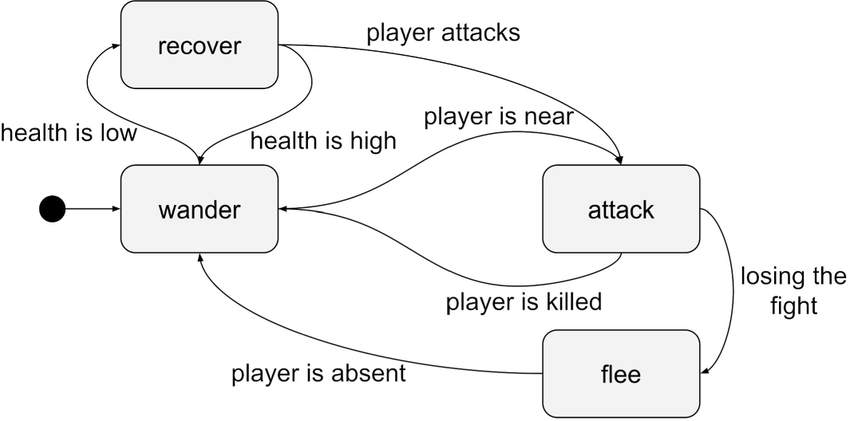
\includegraphics[width=0.7\textwidth]{images/fsm.png}
    \caption{Schemat maszyny stanów dla postaci NPC \cite{Fsm_image}.}
    \label{fig:fsm}
\end{figure}

\subsection{Przykłady stanów}
\subsubsection*{Idle}

W stanie \textbf{Idle} NPC nic nie robi, ale regularnie sprawdza, 
czy gracz nie znalazł się w jego polu widzenia. 
Jeżeli tak, przechodzi do stanu \textbf{Chase}.

\begin{lstlisting}[language=C++, caption={Stan Idle}, label={lst:fsm_idle}]
if (seePlayer()) {
    state = State::Chase;
}
else {
    wait();
}
\end{lstlisting}

\subsubsection*{Patrol}

W stanie \textbf{Patrol} NPC porusza się pomiędzy punktami wyznaczonymi na mapie. 
Jeżeli zauważy gracza — przechodzi do stanu \textbf{Chase}.

\begin{lstlisting}[language=C++, caption={Stan Patrol}, label={lst:fsm_patrol}]
moveTo(nextWaypoint());

if (seePlayer()) {
    state = State::Chase;
}
\end{lstlisting}

\subsubsection*{Chase}

W stanie \textbf{Chase} NPC biegnie w stronę gracza. 
Jeżeli odległość do gracza jest mała — zmienia stan na \textbf{Attack}, 
a jeżeli gracz ucieknie z zasięgu widzenia — powraca do stanu \textbf{Return}.

\begin{lstlisting}[language=C++, caption={Stan Chase}, label={lst:fsm_chase}]
moveTowards(player.position);

if (distanceTo(player) < ATTACK_RANGE) {
    state = State::Attack;
}
else if (!seePlayer()) {
    state = State::Return;
}
\end{lstlisting}

\subsubsection*{Attack}

W stanie \textbf{Attack} NPC wykonuje animację ataku i zadaje obrażenia graczowi. 
Jeżeli gracz oddali się poza zasięg, NPC wraca do stanu \textbf{Chase}.

\begin{lstlisting}[language=C++, caption={Stan Attack}, label={lst:fsm_attack}]
performAttack(player);

if (distanceTo(player) > ATTACK_RANGE) {
    state = State::Chase;
}
\end{lstlisting}

FSM pozwala w prosty sposób zorganizować zachowanie przeciwników 
i jest intuicyjny nawet dla osób nietechnicznych. 
Każdy stan można traktować jak \textit{rolę}, którą odgrywa postać: 
stanie, patroluje, goni lub atakuje. 
Przejścia pomiędzy stanami przypominają decyzje w codziennym życiu 
— np.\ „jeżeli widzę zagrożenie, uciekam; jeżeli go nie ma, odpoczywam”.

\chapter{Implementacja algorytmów w Unity}

\textbf{Silnik gier komputerowych} (ang.\ \texttt{game engine}) to specjalistyczne środowisko programistyczne, 
które dostarcza zestaw narzędzi i bibliotek ułatwiających tworzenie gier. 
Silnik odpowiada za obsługę wielu podstawowych zadań technicznych, 
takich jak grafika, fizyka, dźwięk, sztuczna inteligencja czy interakcja z graczem \cite{GameEngines}.
\section{Wprowadzenie do platformy Unity}

\textbf{Unity} to jeden z najpopularniejszych silników gier komputerowych, 
używany do tworzenia projektów w 2D, 3D, VR oraz AR. 
Powstał w 2005 roku, a obecnie jest dostępny w wersji \textbf{Unity 6.0} \cite{Unity_Manual}. 
Silnik zapewnia zarówno narzędzia edytora (wizualne budowanie sceny, import zasobów, zarządzanie komponentami), 
jak i pełne wsparcie dla programowania logiki w języku \textbf{C\#}.  

Unity opiera się na \textbf{komponentowym modelu programowania} (ang.\ \texttt{component-based programming}). 
Oznacza to, że każdy obiekt w scenie (GameObject) 
jest „pustym kontenerem”, do którego można przypisywać komponenty, nadające mu określone cechy i zachowania. 
Na przykład ten sam GameObject może stać się kamerą, światłem albo postacią gracza --- 
wystarczy dodać odpowiednie komponenty.  

\subsection{Łączenie komponentów}

Dzięki łączeniu komponentów Unity pozwala budować złożone obiekty.  
Przykład: aby stworzyć postać gracza, możemy użyć:
\begin{enumerate}
  \item GameObject z komponentem Transform,
  \item komponent graficzny (np.\ MeshRenderer, SpriteRenderer),
  \item komponent światła (opcjonalnie, np.\ latarka w ręce gracza),
  \item własny skrypt (logika ruchu i interakcji).
\end{enumerate}

Wszystkie niezbędne komponenty zostaną szczegółowo omówione w dalszych rozdziałach, w kontekście ich praktycznego zastosowania.  

\subsection{Skrypty i MonoBehaviour}

Jedną z największych zalet Unity jest możliwość pisania własnych skryptów w języku C\#.  
Skrypty dodaje się do obiektu w taki sam sposób, jak każdy inny komponent --- 
po ich przypisaniu stają się częścią logiki GameObjectu.  

Podstawą dla wszystkich skryptów jest klasa \textbf{MonoBehaviour} \cite{MonoBehaviour}. 
Dziedziczenie po niej umożliwia korzystanie z tzw. \textbf{cyklu życia obiektu}, 
czyli wbudowanych metod wywoływanych automatycznie przez silnik, np.:
\begin{itemize}
  \item \texttt{Start()} — wywoływana raz, przy pierwszej aktywacji obiektu,
  \item \texttt{Update()} — wywoływana co klatkę, odpowiednia do sterowania ruchem czy animacją,
  \item \texttt{OnCollisionEnter2D()} — wywoływana, gdy obiekt wejdzie w kolizję (w kontekście 2D).
\end{itemize}

\begin{lstlisting}[language=C++, caption={Przykład prostego skryptu ruchu w Unity (C\#)}, label={lst:unity_move}]
using UnityEngine;

public class PlayerMovement : MonoBehaviour {
    public float speed = 5f; // parametr do ustawienia w edytorze

    void Update() {
        float moveX = Input.GetAxis("Horizontal");
        float moveY = Input.GetAxis("Vertical");
        transform.position += new Vector3(moveX, moveY, 0) *
        speed * Time.deltaTime;
    }
}
\end{lstlisting}

W powyższym przykładzie:
\begin{itemize}
  \item parametr \texttt{speed} można ustawić ręcznie w edytorze Unity,
  \item metoda \texttt{Update()} jest wywoływana automatycznie co klatkę,
  \item skrypt manipuluje komponentem \texttt{Transform}, zmieniając pozycję gracza.  
\end{itemize}

Tego typu podejście sprawia, że programista nie musi pisać od zera całej logiki renderowania czy wejścia użytkownika — 
wystarczy nadpisać wybrane metody cyklu życia obiektu.  

\subsection{Porównanie z innymi silnikami gier}

Unity nie jest jedynym środowiskiem do tworzenia gier komputerowych. 
W praktyce deweloperzy wybierają spośród kilku najpopularniejszych silników, 
z których najważniejsze to \textbf{Unreal Engine} oraz \textbf{Godot}. 
Każdy z nich posiada swoje mocne i słabe strony, a wybór zależy od potrzeb projektu \cite{Unity_Manual, Unreal, Godot}. 

\paragraph{Unreal Engine.}  
Unreal Engine, rozwijany przez firmę Epic Games, 
jest często wybierany przy dużych i realistycznych produkcjach AAA. 
Jego największą zaletą jest zaawansowany system graficzny i narzędzie \textbf{Blueprints}, 
umożliwiające programowanie logiki gry bez kodowania w C++. 
Z drugiej strony, wymaga mocniejszych komputerów i jest bardziej złożony w nauce niż Unity.  

\paragraph{Godot.}  
Godot to silnik otwartoźródłowy, dostępny na licencji MIT. 
Cechuje się lekkością, prostotą i szybkim prototypowaniem. 
Własny język skryptowy \textbf{GDScript} przypomina Python, 
a od wersji 4.0 wspierane są także C\# i C++. 
Godot jest szczególnie popularny wśród niezależnych twórców, 
ale ma mniej rozbudowany ekosystem niż Unity czy Unreal.  

\paragraph{Unity.}  
Unity zajmuje pozycję pośrednią: 
jest bardziej przystępny niż Unreal, 
a jednocześnie bogatszy w narzędzia i zasoby niż Godot. 
Dzięki obsłudze wielu platform (PC, konsole, urządzenia mobilne, VR/AR) 
często wybierany jest do projektów komercyjnych i edukacyjnych.

Unity zapewnia balans pomiędzy prostotą a możliwościami. 
Unreal lepiej sprawdza się w produkcjach wysokobudżetowych, 
w których kluczowa jest grafika i realizm, 
natomiast Godot jest świetnym wyborem do szybkiego prototypowania i projektów niezależnych. 
Dzięki swojej elastyczności Unity znajduje zastosowanie zarówno w edukacji, 
jak i w komercyjnych projektach różnych gatunków gier. 


\subsection*{Podsumowanie}

Unity jest elastycznym i potężnym środowiskiem, 
które łączy wizualny edytor sceny z programowaniem w języku C\#.  
Kluczowe idee to:
\begin{itemize}
  \item \textbf{GameObject jako kontener} — każdy obiekt sceny składa się z komponentów,
  \item \textbf{komponenty jako funkcjonalności} — można je swobodnie dodawać, usuwać i konfigurować,
  \item \textbf{skrypty oparte na MonoBehaviour} — nadają indywidualną logikę i reagują na cykl życia gry,
  \item \textbf{modularność} — Unity pozwala na szybkie prototypowanie i rozwój gier w różnych gatunkach.
\end{itemize}


\section{Opis zaimplementowanej gry}

Zaimplementowana gra składa się z dwóch głównych etapów: 
\textbf{edycji (editing)} oraz \textbf{symulacji (simulation)}. 
Pierwszy z nich pozwala graczowi przygotować scenę gry poprzez rysowanie i rozmieszczanie obiektów, 
drugi natomiast uruchamia logikę sztucznej inteligencji oraz interakcje pomiędzy obiektami.  

\subsection{Etap I: Edytowanie}

Na etapie edycji gracz posiada możliwość \textbf{tworzenia własnych obiektów} oraz ich \textbf{rozmieszczania na siatce Tilemap}.  
\textbf{Tilemap} to system kafelków wbudowany w Unity, który dzieli scenę na regularną siatkę kwadratowych pól (tzw.\ komórek). 
Dzięki temu umieszczanie elementów gry staje się proste i intuicyjne — każdy obiekt zajmuje dokładnie jedną komórkę mapy.  

Rodzaje obiektów, które mogą zostać dodane w tym etapie, to:
\begin{itemize}
    \item \textbf{Physical object} — prosty obiekt fizyczny bez logiki. Jest to jedynie model 3D lub sprite 2D, 
    który zajmuje pole na mapie i może blokować ruch innych postaci. Nie przechowuje żadnych danych ani funkcji.  

    \item \textbf{Player} — obiekt głównego bohatera gry. Zawiera model, logikę ruchu oraz możliwość interakcji z innymi obiektami. 
    W grze może istnieć tylko \textbf{jedna instancja gracza}.  

    \item \textbf{NPC (Non-Player Character)} — obiekt sterowany przez prymitywną sztuczną inteligencję, 
    opartą na maszynie stanów skończonych (FSM). Każdy NPC posiada własny model i podstawową logikę reakcji na działania gracza.  
\end{itemize}

Na tym etapie główny nacisk kładziony jest na \textbf{logikę rysowania i wycinania modeli}, 
które następnie mogą być osadzane na siatce Tilemap, aby utworzyć unikalne środowisko gry. 


\begin{figure}[H]
    \centering
    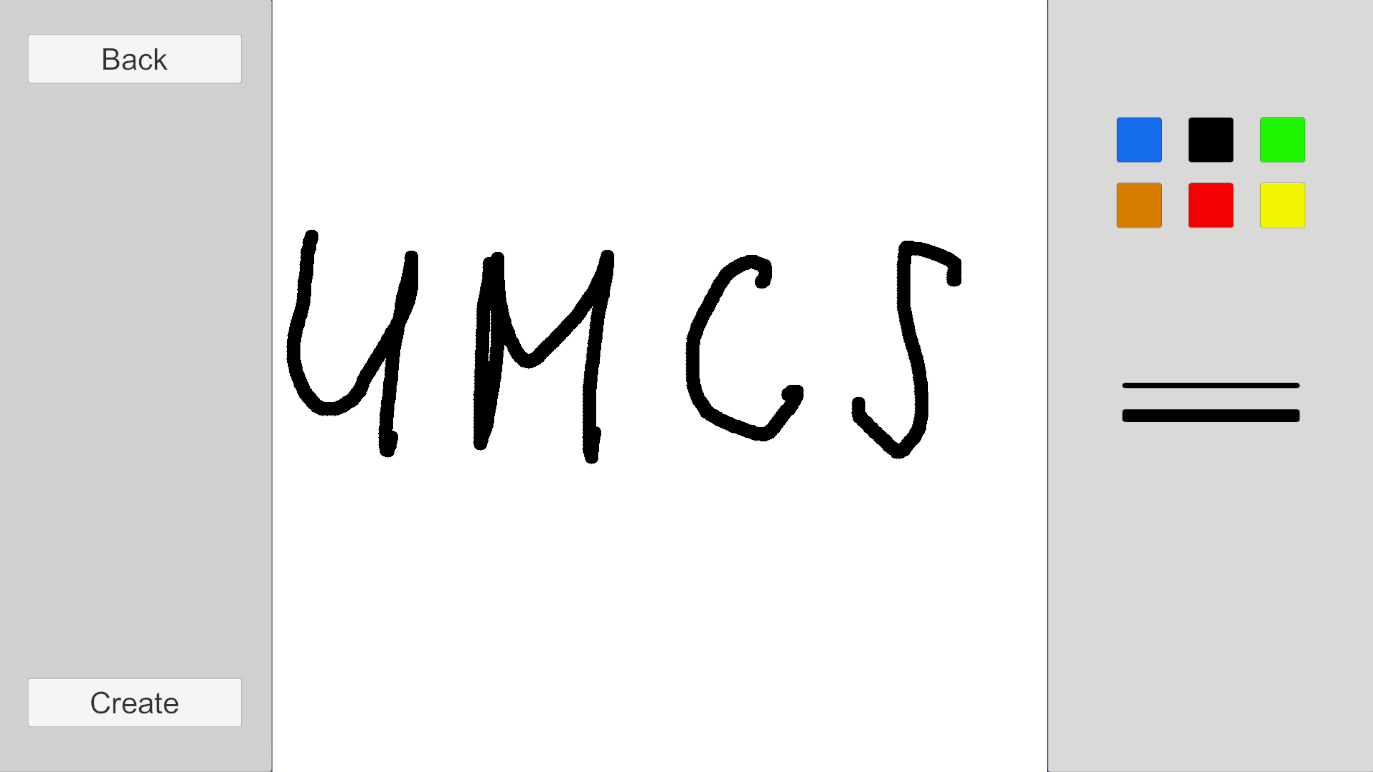
\includegraphics[width=0.7\textwidth]{images/drawingpanel.png}
    \caption{Etap edycji --- panel rysowania}
    \label{fig:drawing_panel}
\end{figure}

\begin{figure}[H]
    \centering
    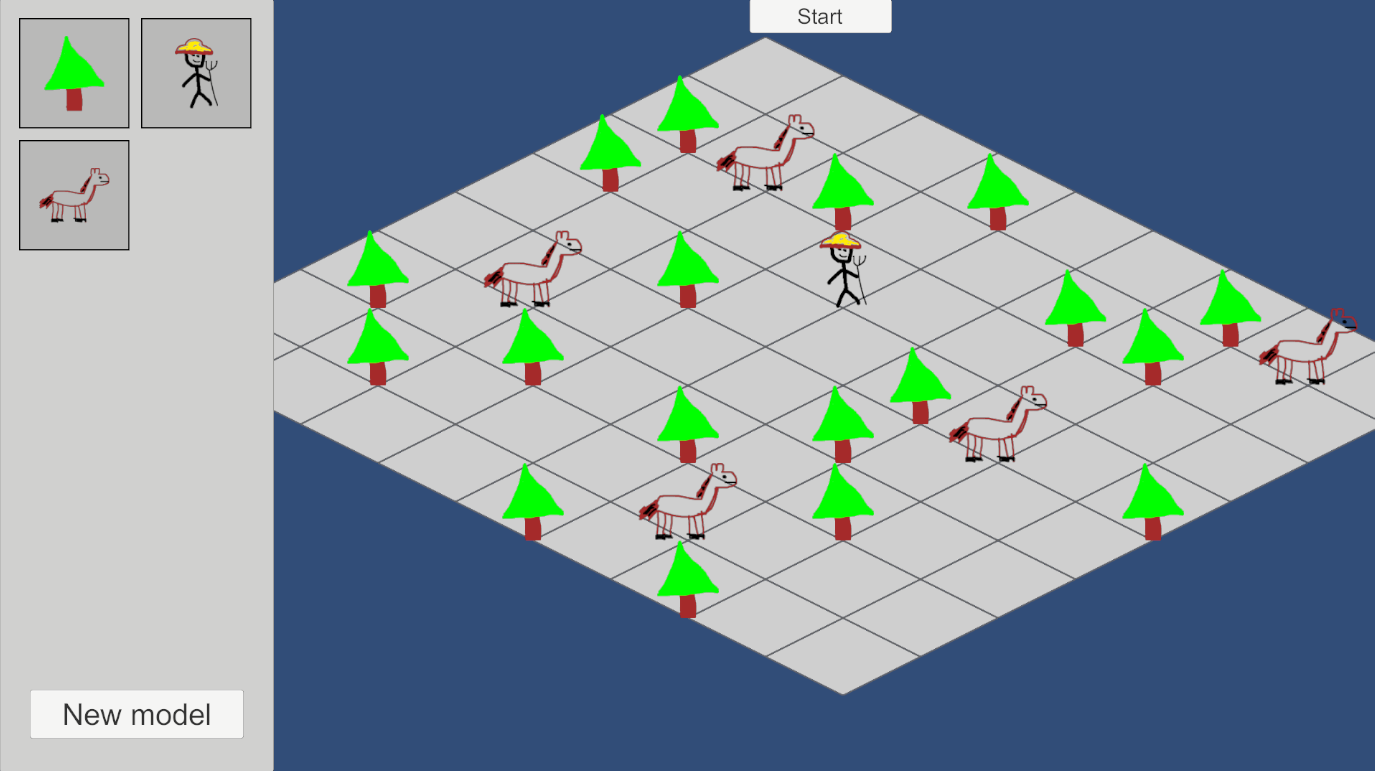
\includegraphics[width=0.7\textwidth]{images/editmode.png}
    \caption{Etap edycji — przykładowe rozmieszczanie obiektów na siatce Tilemap.}
    \label{fig:editing_stage}
\end{figure}

\subsection{Etap II: Symulacja}

Drugi etap to właściwa \textbf{symulacja rozgrywki}. 
Na tym etapie aktywowana zostaje logika wszystkich „żywych” obiektów, tj.\ gracza i NPC.  

\begin{itemize}
    \item \textbf{NPC} — każdy obiekt sterowany przez sztuczną inteligencję funkcjonuje w oparciu o FSM z trzema stanami:
    \begin{itemize}
        \item \texttt{Idle} --- postać stoi w miejscu i obserwuje otoczenie,  
        \item \texttt{Patrol} --- NPC porusza się po wyznaczonej trasie,  
        \item \texttt{Flee} --- NPC ucieka, jeśli gracz go „przegoni”.  
    \end{itemize}
    Przejścia między stanami zachodzą automatycznie w zależności od działań gracza i warunków na mapie.
    
    \item \textbf{Player} — gracz może poruszać się po mapie (ruch w obrębie Tilemap), 
    a dodatkowo posiada możliwość \textbf{przepędzania NPC}. 
    Interakcja polega na kliknięciu w model NPC, co wyzwala przejście jego FSM do stanu \texttt{Flee}.
\end{itemize}



Na tym etapie realizowane są również \textbf{algorytmy sztucznej inteligencji i fizyki}, w tym:
\begin{itemize}
    \item algorytm wyszukiwania ścieżki \textbf{A*},  
    \item \textbf{FSM} jako logika NPC,  
    \item \textbf{wykrywanie kolizji}, pozwalające na prawidłowe interakcje pomiędzy obiektami.  
\end{itemize}

Gra łączy w sobie dwa etapy: \textbf{etap kreatywny} (edycja, rysowanie i rozmieszczanie obiektów) 
oraz \textbf{etap dynamiczny} (symulacja z logiką gracza i NPC). 
Takie podejście pozwala użytkownikowi zarówno na tworzenie własnego środowiska, 
jak i na jego eksplorację oraz interakcję z obiektami. 
Dzięki zastosowaniu FSM i algorytmu A* zachowanie postaci niezależnych jest przewidywalne, ale jednocześnie dynamiczne, 
co czyni rozgrywkę ciekawszą i bardziej angażującą.

\section{Wyznaczanie pozycji kursora w Unity}

Zanim, jak zaczniemy analizować zaimplementowane algorytmy, warto zwrócić uwagę na mechanizm wyznaczania pozycji kursoru w przestrzeni świata w Unity.

W procesie rysowania istotne jest ustalenie, gdzie dokładnie znajduje się kursor gracza w danym momencie. 
Unity udostępnia wbudowane mechanizmy, które automatycznie przeliczają pozycję myszy na odpowiednie współrzędne --- programista nie musi wykonywać skomplikowanych obliczeń ręcznie.  

\paragraph{Od ekranu do obiektu}
Na początku pozycja kursora istnieje w tak zwanej \emph{przestrzeni ekranu}, czyli w pikselach monitora. 
Unity potrafi przekształcić te wartości na współrzędne odpowiedniego obiektu w grze. 
Na przykład w naszym przypadku rysujemy na obiekcie \textbf{Raw Image}, który jest częścią interfejsu użytkownika (UI). 
Silnik automatycznie wylicza, gdzie dokładnie w obrębie tego elementu znajduje się kursor i pozwala wskazać piksel tekstury, który należy zmienić.

\paragraph{Rola kamery}
Transformacja współrzędnych kursora zależy również od \textbf{kamery}, ponieważ to właśnie ona „patrzy” na scenę i wyznacza, jak ekran odwzorowuje przestrzeń gry.  
Unity samo dba o to, aby uwzględnić ustawienia kamery (jej pozycję, tryb rzutowania czy odległość od obiektów). 
W praktyce oznacza to, że programista wywołuje jedną funkcję, a silnik zajmuje się wszystkimi obliczeniami w tle.

\paragraph{Dlaczego odległość jest ważna?}
W grach trójwymiarowych ten sam punkt na ekranie może odpowiadać wielu różnym punktom w świecie gry (na różnych głębokościach). 
Dlatego istotne jest, na jakiej odległości od kamery znajduje się obiekt, który chcemy wskazać.  
Unity również to uwzględnia automatycznie: dla interfejsu 2D (takiego jak nasze rysowanie na \texttt{Raw Image}) dystans nie ma znaczenia, a w przypadku obiektów 3D silnik sam oblicza, który element został kliknięty, często korzystając z mechanizmu \emph{raycastu}.

Cały proces sprowadza się więc do prostego zapytania: „gdzie znajduje się kursor względem mojego obiektu?”.  
Unity wykonuje wszystkie przeliczenia automatycznie — bierze pod uwagę ekran, kamerę, odległości i przekształca je na współrzędne, które możemy wykorzystać np.\ do rysowania pikseli na teksturze. 
Dzięki temu programista nie musi znać szczegółów matematycznych, a jedynie używa odpowiedniej funkcji wbudowanej w silnik.


\section{Implementacja metody rysowania}

W zaimplementowanej grze powstał mechanizm malowania na panelu edycyjnym. 
Umożliwia on:
\begin{itemize}
  \item rysowanie kół o zadanej średnicy,
  \item łączenie kolejnych kół w linię ciągłą,
  \item wybieranie szerokości i koloru linii,
  \item korzystanie z trybu gumki.
\end{itemize}

Do realizacji rysowania zostały wykorzystane następujące komponenty Unity:
\begin{itemize}
  \item \textbf{Raw Image} --- obiekt UI, do którego przypisana zostaje tekstura, na której gracz rysuje.
  \item \textbf{Texture2D} --- dynamiczna tekstura, na której zmieniane są piksele podczas rysowania.
  \item \textbf{RectTransform} komponentu Raw Image --- służy do przekształcenia współrzędnych kursora (ekranowych) na współrzędne tekstury.
\end{itemize}


\subsection{Rysowanie koła}

Pierwsza funkcjonalność to rysowanie wypełnionego koła na podstawie równania:
\[
x^2 + y^2 \leq r^2
\]
gdzie \(r\) to promień koła.  
Dla każdego piksela sprawdzane jest, czy należy do obszaru koła, a jeśli tak — zostaje pokolorowany.

\begin{lstlisting}[language=CSharp, caption={Funkcja DrawCircle}, label={lst:drawcircle}]
// Funkcja rysuje wypelnione kolo na teksturze
private void DrawCircle(int x, int y)
{
    for (int i = -drawingLine.size; i < drawingLine.size; i++)
    {
        for (int j = -drawingLine.size; j < drawingLine.size; j++)
        {
            // sprawdzamy czy punkt lezy w obrebie kola
            if (i * i + j * j <= drawingLine.size * drawingLine.size)
            {
                int pixelX = x + i;
                int pixelY = y + j;
                
                // jesli piksel znajduje sie w granicach tekstury
                if (pixelX >= 0 && pixelX < texture.width &&
                    pixelY >= 0 && pixelY < texture.height) 
                {
                    texture.SetPixel(pixelX, pixelY, drawingLine.color);
                }
            }
        }
    }
}
\end{lstlisting}

Szerokość i kolor linii definiowane są przez obiekt \textbf{DrawingLineSO}. 
Wartości te można edytować w panelu inspektora po prawej stronie edytora Unity.

\begin{figure}[H]
    \centering
    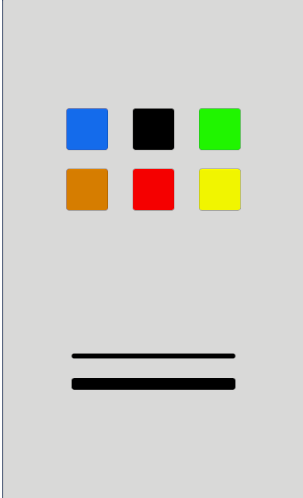
\includegraphics[width=0.4\textwidth]{images/inspectorpanel.png}
    \caption{Panel inspektora}
    \label{fig:editing_stage}
\end{figure}

\subsection{Rysowanie linii}

Linia rysowana jest jako ciąg małych kół (pociągły „pędzel”) wzdłuż wektora od punktu początkowego do końcowego.  
Dzięki temu powstaje gładka, ciągła kreska.

\begin{lstlisting}[language=CSharp, caption={Funkcja DrawLine}, label={lst:drawline}]
// Funkcja rysuje linie poprzez interpolacje punktow
private void DrawLine(Vector2 start, Vector2 end)
{
    float distance = Vector2.Distance(start, end);
    Vector2 direction = (end - start).normalized;

    // co 5 pikseli rysujemy kolo
    for (float i = 0; i < distance; i += 5f)  
    { 
        Vector2 position = start + direction * i;
        DrawCircle((int)position.x, (int)position.y);
    }
    
    texture.Apply(); // aktualizacja zmian
}
\end{lstlisting}

\subsection{Metoda Update}

Funkcja \texttt{Update} w Unity uruchamiana jest automatycznie raz na każdą klatkę (\textit{frame per second}). 
Odpowiada za sprawdzanie, czy gracz przytrzymuje przycisk myszy i czy w danym momencie należy narysować koło lub linię. 
Warto podkreślić, że częstotliwość wywołania \texttt{Update} zależy od liczby klatek na sekundę, co może wpływać na wrażenia z rysowania (płynność, gęstość próbkowania punktów).

\begin{lstlisting}[language=CSharp, caption={Fragment metody Update}, label={lst:update}]
// Funkcja wykonywana raz na kazda klatke
private void Update()
{
    if (Input.GetMouseButton(0))
    {
        // pobieramy pozycje kursora w przestrzeni ekranu
        Vector2 mousePosition;
        RectTransformUtility.ScreenPointToLocalPointInRectangle(
        rectTransform, Input.mousePosition, Camera.main, out mousePosition);

        // przesuwamy wspolrzedne aby odpowiadaly teksturze
        mousePosition.x += rectTransform.rect.width / 2;
        mousePosition.y += rectTransform.rect.height / 2;

        // sprawdzamy czy pozycja jest w granicach tekstury
        if (mousePosition.x >= 0 && mousePosition.y >= 0 &&
            mousePosition.x < rectTransform.rect.width &&
            mousePosition.y < rectTransform.rect.height)
        {
            if (lastMousePosition == null)
            {
                DrawCircle((int)mousePosition.x, (int)mousePosition.y);
            }
            else if (Vector2.Distance((Vector2)lastMousePosition, mousePosition)
            >= pointOffset)
            {
                DrawLine((Vector2)lastMousePosition, mousePosition);
            }
            
            lastMousePosition = mousePosition;
        }
        else
        {
            lastMousePosition = null;
        }
    }

    // reset po puszczeniu przycisku myszy
    if (Input.GetMouseButtonUp(0))
    {
        lastMousePosition = null;
    }

    // zmiana trybu na gumke (Q)
    if (Input.GetKeyDown(KeyCode.Q))
    {
        drawingLine.ToggleEraserMode();
    }
}
\end{lstlisting}

Tryb gumki to ten sam algorytm rysowania, z tą różnicą, że aktualny kolor pędzla ustawiany jest na przezroczysty (\texttt{Color.clear}). 
W praktyce „rysujemy” wtedy przezroczystością, wymazując fragment obrazu.

Algorytm rysowania został zaimplementowany w oparciu o rysowanie kół i interpolację linii. 
Dzięki dynamicznej teksturze przypiętej do \textbf{Raw Image} gracz może swobodnie rysować na panelu edycyjnym, 
zmieniać szerokość i kolor kreski oraz korzystać z gumki. 
Rozwiązanie jest elastyczne, proste w implementacji i dobrze wpisuje się w komponentowy model Unity.

\section{Tworzenie niestandardowych koliderów}

Po tym, jak gracz narysował swoją modelkę, następnym krokiem jest jej \textbf{przycięcie} (wycięcie minimalnego prostokąta otaczającego rysunek). Na podstawie tak uzyskanej obwiedni (ang.\ \emph{bounding box}) tworzymy \textbf{Box Collider 2D}, który będzie używany do wykrywania kliknięć kursorem w modelki oraz do dalszych interakcji w grze.

Przycinanie polega na odnalezieniu granic wszystkich nieprzezroczystych pikseli (kanał alfa) i wycięciu z oryginalnej tekstury tylko tego fragmentu, który zawiera narysowany obiekt. Minimalizuje to rozmiar danych i pozwala jednoznacznie określić rozmiar kolidera. Box Collider 2D dopasowany do obwiedni sprawia, że kliknięcie kursorem oraz inne testy kolizji działają precyzyjnie.

\begin{lstlisting}[language=CSharp, caption={Przycinanie tekstury do obszaru narysowanego obiektu}, label={lst:filtertexture}]
private Texture2D FilterTexture(Texture2D source) 
{
    int width = source.width;
    int height = source.height;

    // poczatkowe wartosci granic
    int xMin = width, xMax = 0, yMin = height, yMax = 0;

    // pobieramy wszystkie piksele tekstury
    Color[] pixels = source.GetPixels();

    // przechodzimy po calej teksturze
    for (int y = 0; y < height; y++) {
        for (int x = 0; x < width; x++) {
            Color pixel = pixels[y * width + x];

            // sprawdzamy czy piksel jest nieprzezroczysty
            if (pixel.a != 0) {
                if (x < xMin) xMin = x;
                if (x > xMax) xMax = x;
                if (y < yMin) yMin = y;
                if (y > yMax) yMax = y;
            }
        }
    }

    // obliczamy wymiary nowego wycinka
    int newWidth = xMax - xMin + 1;
    int newHeight = yMax - yMin + 1;

    // kopiujemy piksele tylko z obszaru obiektu
    Color[] newPixels = source.GetPixels(xMin, yMin, newWidth, newHeight);

    // tworzymy nowa teksture z wycinka
    Texture2D croppedTexture = new Texture2D(newWidth, newHeight, 
                                             TextureFormat.RGBA32, true);
    croppedTexture.SetPixels(newPixels);
    croppedTexture.Apply();

    return croppedTexture;
}
\end{lstlisting}

\subsection*{Utrwalenie modelki i prefab z podziałem na „zewnętrzne” i „wewnętrzne”}

Po utworzeniu „zewnętrznego” wyglądu modelki (czyli przyciętej tekstury/sprite’a), zapamiętujemy ten obiekt w pamięci programu. Dzięki temu gracz może w dowolnym momencie \textbf{umieścić} go na siatce zgodnie z wybranym \textbf{typem obiektu} (np.\ Physical object, Player, NPC).

Do utworzenia gotowego obiektu w świecie gry wykorzystujemy \textbf{prefab}, czyli gotowy szablon objeku, który rozdziela:
\begin{itemize}
  \item \textbf{object sprite} --- warstwa „zewnętrzna” (wygląd): renderer ze sprite’em/teksturą,
  \item \textbf{object data} --- warstwa „wewnętrzna” (logika/dane): komponenty skryptowe, identyfikator typu, parametry obiektu itp.
\end{itemize}
W momencie składania finalnego obiektu \emph{generujemy Box Collider 2D} na podstawie przyciętej modelki (jej rozmiaru). Kolider bywa umieszczany na dziecku prefabu (części graficznej), dlatego praktycznym wzorcem jest pobieranie go z potomków.

\subsection*{Ustawienie rozmiaru kolidera na podstawie sprite’a}

Po wstawieniu sprite’a do \emph{object sprite} ustawiamy rozmiar \textbf{BoxCollider2D} zgodnie z rozmiarem renderowanego sprite’a (w jednostkach świata):

\begin{lstlisting}[language=CSharp, caption={Dopasowanie rozmiaru Box Collider 2D do sprite’a}, label={lst:setcollider}]
obj.GetComponentInChildren<BoxCollider2D>().size = 
spriteRenderer.bounds.size;
\end{lstlisting}

\noindent Krótkie wyjaśnienie elementów powyższej instrukcji:
\begin{itemize}
  \item \texttt{obj} — instancja naszego prefabu w scenie (obiekt nadrzędny),
  \item \texttt{GetComponentInChildren<BoxCollider2D>()} — pobiera komponent kolidera typu \texttt{BoxCollider2D} z obiektu \emph{dziecka} (tam, gdzie mamy część graficzną),
  \item \texttt{spriteRenderer} — odwołanie do komponentu \texttt{SpriteRenderer} (część „zewnętrzna”),
  \item \texttt{spriteRenderer.bounds.size} — wektor 2D/3D reprezentujący \textbf{rozmiar sprite’a w jednostkach świata} (po skalowaniu); używamy go, aby kolider miał dokładnie taki sam rozmiar jak widoczny obraz.
\end{itemize}

Dzięki temu kliknięcia myszą oraz inne testy kolizyjne będą działały spójnie z tym, co widzi gracz.

\subsection*{Złożoność obliczeniowa}

Koszt obliczeniowy przycinania tekstury jest liniowy względem liczby pikseli:
\[
O(W \cdot H),
\]
ponieważ skanujemy każdy piksel raz, aby wyznaczyć obwiednię. Kopiowanie wycinka to również koszt liniowy względem rozmiaru wycinka. Złożoność pamięciowa jest liniowa (przechowujemy tablicę pikseli wejściowych oraz pikseli wycinka). Operacja ustawienia rozmiaru kolidera jest stałokosztowa:
\[
O(1).
\]

W pierwszym kroku obcinamy teksturę do minimalnego prostokąta zawierającego rysunek, a następnie tworzymy prefab, który rozdziela wygląd (\emph{object sprite}) od danych/logiki (\emph{object data}). Na podstawie rozmiaru sprite’a automatycznie dopasowujemy \textbf{Box Collider 2D}, co zapewnia zgodność wizualną i poprawne wykrywanie kliknięć. Tak przygotowany obiekt można w dowolnym momencie umieścić na \emph{Tilemap}, zachowując spójność między tym, co widać, a tym, co „czuje” silnik kolizji.

\section{Implementacja algorytmu A*}

Zanim zaczniemy szukać ścieżki, warto przypomnieć, że A* działa na \textbf{grafie}: zbiorze punktów (wierzchołków) połączonych możliwymi przejściami (krawędziami) z przypisanym kosztem ruchu. W naszej grze takim grafem staje się \emph{siatka} Tilemap: każda komórka to wierzchołek, a przejścia prowadzą do sąsiadów. Żeby A* mógł pracować, najpierw musimy zbudować w pamięci programu prostą reprezentację, która mówi, które komórki są przechodnie, a które zablokowane przez przeszkody narysowane wcześniej przez gracza. W praktyce sprowadza się to do ustalenia granic siatki, utworzenia tablicy \emph{walkable} i zaznaczenia w niej pól zajętych przez obiekty fizyczne.

\subsection{Przekształcenie Tilemap w graf (siatkę przechodności)}

Na starcie wyznaczamy położenie i rozmiar używanego obszaru Tilemap, tak aby operować tylko na faktycznie wykorzystywanych kafelkach. Następnie tworzymy dwuwymiarową tablicę wartości logicznych i domyślnie uznajemy wszystkie komórki za dostępne. Potem iterujemy po obiektach sceny i każdy obiekt typu \texttt{PhysicalObject} „rzucamy” na siatkę, aby odszukać jego komórkę. Ta komórka zostaje oznaczona jako niedostępna. Dzięki temu w pamięci mamy gotowy obraz świata: wiemy, po których węzłach wolno chodzić, a które trzeba ominąć. Warto zauważyć, że nie tworzymy tu osobnych list sąsiadów ani struktur krawędzi --- siatka jest regularna, więc sąsiedztwo wyznaczymy na bieżąco podczas działania A*.

\begin{lstlisting}[language=CSharp, caption={Budowa siatki przechodnosci na podstawie Tilemap i obiektow}, label={lst:walkablegrid_easy}]
private void Awake()
{
    Instance = this; // prosty singleton

    CalculateGridBounds();
    GenerateWalkableGrid();
}

void CalculateGridBounds()
{
    tilemap.CompressBounds(); // zawija do faktycznie uzywanych kafelkow
    gridOrigin = tilemap.cellBounds.position; // lewy dolny rog w ukladzie
                                              // komorek
    gridSize = tilemap.cellBounds.size;     // rozmiar siatki w komorkach
}

public void GenerateWalkableGrid()
{
    walkableGrid = new bool[gridSize.x, gridSize.y];

    // najpierw: wszystko dostepne
    for (int x = 0; x < gridSize.x; x++)
        for (int y = 0; y < gridSize.y; y++)
            walkableGrid[x, y] = true;

    // nastepnie blokujemy pola zajete przez obiekty fizyczne
    foreach (GameObject obj in objectFabric.objects)
    {
        if (obj.GetComponentInChildren<ObjectData>().objectData.type != 
        "PhysicalObject")
            continue;

        Vector3 worldPos = obj.transform.position;
        Vector3Int cell  = tilemap.WorldToCell(worldPos);

        int x = cell.x - gridOrigin.x; // mapowanie: komorka -> indeks tablicy
        int y = cell.y - gridOrigin.y;

        if (x >= 0 && y >= 0 && x < gridSize.x && y < gridSize.y)
            walkableGrid[x, y] = false; // to pole jest przeszkoda
    }
}

public bool IsWalkable(Vector3Int cell)
{
    int x = cell.x - gridOrigin.x;
    int y = cell.y - gridOrigin.y;

    if (x < 0 || y < 0 || x >= gridSize.x || y >= gridSize.y)
        return false; // poza plansza traktujemy jako przeszkoda

    return walkableGrid[x, y];
}
\end{lstlisting}

W efekcie przechowujemy graf bardzo oszczędnie: jedna tablica \texttt{walkableGrid} mówi, czy dany wierzchołek (komórka) jest dostępny, a dokładną listę sąsiadów wyprowadzimy z geometrii siatki w chwili obliczeń. Taki model jest prosty, szybki i świetnie pasuje do późniejszego wywoływania A*.

\subsection{Wyszukiwanie ścieżki A* na zbudowanej siatce}

Teraz przechodzimy do samego algorytmu. A* utrzymuje zbiór kandydatów do odwiedzenia, pamięta, skąd przyszliśmy do danego pola, ile nas to dotychczas kosztowało (\(g\)), a także szacuje, ile jeszcze zostało (\(h\)). Suma \(f=g+h\) decyduje o kolejności rozpatrywania węzłów. Poruszamy się o jeden krok w pionie, poziomie lub po skosie. Koszt kroku ustawiamy na 10 dla przejść ortogonalnych i 14 dla przekątnych (to praktyczna liczba całkowita zbliżona do \(\sqrt{2}\cdot 10\)). Dzięki temu algorytm wybiera naturalnie „gładkie” trasy, ale jednocześnie nie zezwala na przecinanie rogów — ruch po przekątnej jest możliwy tylko wtedy, gdy oba przyległe pola ortogonalne nie są zablokowane.

\begin{lstlisting}[language=CSharp, caption={Algorytm A* z ruchem po przekatnej i kontrola rogow}, label={lst:astar_easy}]
public class AStarPathfinder : MonoBehaviour
{
    public Tilemap tilemap;

    public List<Vector3Int> FindPath(Vector3Int start, Vector3Int goal)
    {
        var openSet  = new PriorityQueue<Vector3Int>();          
        // kandydaci
        var cameFrom = new Dictionary<Vector3Int, Vector3Int>(); 
        // poprzednicy do rekonstrukcji
        var gScore   = new Dictionary<Vector3Int, int>();        
        // koszt od startu
        var fScore   = new Dictionary<Vector3Int, int>();        
        // g + h

        openSet.Enqueue(start, 0);
        gScore[start] = 0;
        fScore[start] = Heuristic(start, goal);

        while (openSet.Count > 0)
        {
            var current = openSet.Dequeue(); // wierzcholek o najnizszym f

            if (current == goal)
                return ReconstructPath(cameFrom, current);

            foreach (var neighbor in GetNeighbors(current))
            {
                if (!WalkableGridGenerator.Instance.IsWalkable(neighbor)) 
                    continue; // omijamy przeszkody

                int moveCost   = IsDiagonal(current, neighbor) ? 14 : 10;
                int tentativeG = gScore[current] + moveCost;

                if (!gScore.ContainsKey(neighbor) || 
                tentativeG < gScore[neighbor])
                {
                    cameFrom[neighbor] = current;
                    gScore[neighbor]   = tentativeG;
                    fScore[neighbor]   = tentativeG + Heuristic(neighbor, goal);

                    if (!openSet.Contains(neighbor))
                        openSet.Enqueue(neighbor, fScore[neighbor]);
                }
            }
        }

        return null; // gdy brak sciezki
    }

    private List<Vector3Int> GetNeighbors(Vector3Int cell)
    {
        var neighbors = new List<Vector3Int>();
        Vector3Int[] dirs = {
            Vector3Int.up, Vector3Int.down, Vector3Int.left, Vector3Int.right,
            new Vector3Int(-1,  1, 0), new Vector3Int( 1,  1, 0),
            new Vector3Int(-1, -1, 0), new Vector3Int( 1, -1, 0)
        };

        foreach (var d in dirs)
        {
            Vector3Int n = cell + d;

            // brak "ciecia rogow": skos tylko jesli oba 
            //sasiady ortogonalne sa wolne
            if (IsDiagonal(cell, n))
            {
                Vector3Int d1 = new Vector3Int(n.x, cell.y, 0);
                Vector3Int d2 = new Vector3Int(cell.x, n.y, 0);
                if (!WalkableGridGenerator.Instance.IsWalkable(d1) ||
                    !WalkableGridGenerator.Instance.IsWalkable(d2))
                    continue;
            }

            neighbors.Add(n);
        }
        return neighbors;
    }

    // Heurystyka oktalna
    private int Heuristic(Vector3Int a, Vector3Int b)
    {
        int dx = Mathf.Abs(a.x - b.x);
        int dy = Mathf.Abs(a.y - b.y);
        return 10 * (dx + dy) + 4 * Mathf.Min(dx, dy); 
        // 10*(dx+dy) + (14-10)*min
    }

    private bool IsDiagonal(Vector3Int a, Vector3Int b) => 
        a.x != b.x && a.y != b.y;

    private List<Vector3Int> ReconstructPath
    (Dictionary<Vector3Int, Vector3Int> cameFrom, Vector3Int cur)
    {
        var path = new List<Vector3Int> { cur };
        while (cameFrom.ContainsKey(cur))
        {
            cur = cameFrom[cur];
            path.Insert(0, cur);
        }
        return path;
    }
}
\end{lstlisting}

\subsection*{Użyta heurystyka i dlaczego jest korzystna.}  
W funkcji \texttt{Heuristic} zastosowaliśmy tak zwaną \textbf{heurystykę oktalną}, dopasowaną do ruchu w ośmiu kierunkach z różnymi kosztami: 10 dla ruchu w pionie/poziomie i 14 dla skosu. Intuicyjnie najpierw „płacimy” za część drogi, którą da się pokonać po skosie (to \(\min(dx,dy)\) kroków po 14), a resztę pokonujemy krokami prostymi (to \(|dx-dy|\) kroków po 10). Zapisaliśmy to w prostszej formie całkowitoliczbowej:  
\[
h(a,b) \;=\; 10\cdot(dx+dy)\;+\;4\cdot\min(dx,dy),
\]
co odpowiada \(10|dx-dy| + 14\min(dx,dy)\). Taka heurystyka jest \textbf{admisowalna} (nigdy nie przecenia prawdziwego kosztu) i \textbf{spójna}, więc A* zachowuje optymalność, a jednocześnie przeszukuje znacznie mniej pól niż algorytm Dijkstry. Praktyczna korzyść jest podwójna: ścieżki są \emph{krótsze i gładsze} dzięki dozwolonym przekątnym, a obliczenia — szybsze, bo kierują się „we właściwą stronę” bez zbędnego błądzenia.

\subsection*{Złożoność}

Zbudowanie siatki przechodności polega na jednorazowym przejściu przez wymiary Tilemap i oznaczeniu pól zajętych przez obiekty, co kosztuje tyle, ile liczba komórek plus liczba obiektów. Mówimy więc o czasie \(O(W\cdot H + N_{\text{obiektów}})\) i pamięci \(\Theta(W\cdot H)\) na tablicę \texttt{walkableGrid}. Sam A* na siatce o \(V=W\cdot H\) polach i około \(8V\) możliwych krawędziach ma złożoność rzędu \(O(V\log V)\) przy kolejce priorytetowej i pamięć \(O(V)\) na tablice \(g\), \(f\), poprzedników i zbiór otwarty. W praktyce dobra heurystyka, taka jak zastosowana oktalna, znacząco zmniejsza realną liczbę odwiedzonych pól, więc ścieżki znajdują się szybko nawet na dużych planszach.



Cały proces składa się z dwóch naturalnych kroków. Najpierw „zamieniamy” Tilemap na prostą reprezentację grafu: przechowujemy tylko informację, które komórki są dostępne. Potem uruchamiamy A*: wybieramy zawsze najbardziej obiecującą komórkę według \(f=g+h\), generujemy sąsiadów w ośmiu kierunkach, pilnując, aby nie przecinać rogów, i używamy \textbf{heurystyki oktalnej}, która jest zgodna z przyjętymi kosztami kroków. Dzięki temu obiekt może poruszać się nie tylko w pionie i poziomie, ale również po przekątnej, co daje krótsze, naturalnie wyglądające ścieżki i dobrą wydajność obliczeń.

\section{Stany sztucznej inteligencji i ich opis}

Na potrzeby stworzonej gry została zaimplementowana \textbf{maszyna stanów skończonych (FSM, Finite State Machine)}.  
Przypomnijmy, że FSM to struktura, w której obiekt (w tym przypadku \textit{NPC}) może znajdować się w jednym z kilku zdefiniowanych stanów, a przejścia pomiędzy nimi zależą od określonych warunków.  
Takie podejście pozwala w prosty sposób kontrolować zachowanie przeciwników czy postaci niezależnych, zapewniając przejrzystość i łatwość rozbudowy logiki gry.

\subsection*{Interfejs stanów}

Aby ujednolicić sposób implementacji różnych stanów, został przygotowany interfejs \texttt{INPCState}.  
Dzięki niemu każdy stan posiada trzy metody: \texttt{Enter()} (wywoływana przy wejściu w stan), \texttt{Update()} (uruchamiana co klatkę gry) oraz \texttt{Exit()} (wywoływana przy opuszczaniu stanu).  
Takie rozwiązanie ułatwia organizację kodu i pozwala stosować jeden mechanizm dla różnych zachowań.

\begin{lstlisting}[language=CSharp, caption={Interfejs dla wszystkich stanów NPC}, label={lst:npcstate_interface}]
public interface INPCState
{
    void Enter();   // Wywoluje sie, gdy NPC wchodzi w nowy stan
    void Update();  // Aktualizacja logiki stanu (wykonywana raz na klatke)
    void Exit();    // Wywoluje sie, gdy NPC opuszcza stan
}
\end{lstlisting}

\subsection*{Idle State}

Stan \texttt{Idle} odpowiada za bezczynne oczekiwanie NPC.  
Po wejściu w ten stan NPC zatrzymuje się na losowy czas, wybrany pomiędzy 3 a 8 sekundami.  
Po jego upływie następuje automatyczna zmiana na stan \texttt{Patrol}.  

\begin{lstlisting}[language=CSharp, caption={Implementacja stanu Idle}, label={lst:idle_state}]
public void Enter()
{
    timer = Random.Range(3f, 8f); // Ustawienie losowego czasu oczekiwania
}

public void Exit()
{
    timer = 0f; // Zerowanie timera po opuszczeniu stanu
}

public void Update()
{
    timer -= Time.deltaTime; // Odliczanie czasu
    if (timer <= 0)
    {
        npc.stateMachine.ChangeState(new PatrolState(npc));
    }
}
\end{lstlisting}

\subsection*{Patrol State}

Stan \texttt{Patrol} powoduje, że NPC zaczyna poruszać się losowo po mapie w wyznaczonym promieniu od swojej pozycji.  
Do obliczania ścieżki ponownie wykorzystywany jest zaimplementowany wcześniej algorytm \textbf{A*}.  
Dodatkowo została przygotowana funkcja losująca punkt docelowy w zadanym promieniu, co nadaje NPC wrażenie bardziej naturalnego zachowania.  

\begin{lstlisting}[language=CSharp, caption={Implementacja stanu Patrol}, label={lst:patrol_state}]
public void Enter()
{
    // Pobranie referencji do niezbednych komponentow
    pathfinder = GameObject.Find("AStarPathfinder")
    .GetComponent<AStarPathfinder>();
    tilemap = GameObject.Find("Tilemap").GetComponent<Tilemap>();
    walkableGridGenerator = GameObject.Find("WalkableGridGenerator")
    .GetComponent<WalkableGridGenerator>();
    pathWorld = new();

    // Wyznaczenie aktualnej pozycji NPC w siatce
    Vector3Int npcCell = tilemap.WorldToCell(npc.transform.position);

    // Wybieramy losowy punkt docelowy w poblizu NPC
    List<Vector3Int> destinationCells = 
    walkableGridGenerator.GetRandomWalkableCellAround(npcCell, patrolRadius);

    foreach(var destination in destinationCells)
    {
        List<Vector3Int> path = pathfinder.FindPath(npcCell, destination);
        if (path != null)
        {
            pathWorld.Clear();
            foreach (var cell in path)
                pathWorld.Add(tilemap.GetCellCenterWorld(cell));

            pathIndex = 0;
            destinationCell = destination;
            return;
        }
    }
}

public void Update()
{
    MoveAlongPath(); // Ruch wzdluz wyznaczonej sciezki
}
\end{lstlisting}

Funkcja odpowiedzialna za wybór losowego punktu w promieniu:

\begin{lstlisting}[language=CSharp, caption={Losowanie punktu patrolu}, label={lst:random_walkable}]
public List<Vector3Int> GetRandomWalkableCellAround
(Vector3Int position, int radius)
{ 
    List<Vector3Int> candidates = new();

    for (int dx = -radius; dx <= radius; dx++)
    {
        for (int dy = -radius; dy <= radius; dy++)
        {
            Vector3Int candidate = 
            new Vector3Int(position.x + dx, position.y + dy, 0);

            if (!IsWalkable(candidate)) continue;

            int x = candidate.x - gridOrigin.x;
            int y = candidate.y - gridOrigin.y;

            if (x >= 0 && y >= 0 && x < gridSize.x && y < gridSize.y)
            {
                candidates.Add(candidate);
            }
        }
    }

    if (candidates.Count == 0)
        return new List<Vector3Int> { position };

    candidates = Shuffle(candidates); // Losowe przemieszanie
    return candidates;
}
\end{lstlisting}

\subsection*{Flee State}

Stan \texttt{Flee} aktywuje się w momencie, gdy gracz kliknie w model NPC.  
Postać zaczyna wtedy uciekać w przeciwną stronę od pozycji gracza.  
Ponownie wykorzystywany jest algorytm A*, natomiast dodatkowo zaimplementowano mechanizm wyboru punktu docelowego w przeciwnym kierunku względem gracza.  

\begin{lstlisting}[language=CSharp, caption={Implementacja stanu Flee}, label={lst:flee_state}]
public void Enter()
{
    Vector3Int npcCell = tilemap.WorldToCell(npc.transform.position);
    Vector3Int threatCell = tilemap.WorldToCell(npc.player.transform.position);

    fleePath = CalculateFleePath(npcCell, threatCell);

    if (fleePath != null)
    {
        pathWorld = new List<Vector3>();
        foreach (var cell in fleePath)
            pathWorld.Add(tilemap.GetCellCenterWorld(cell));

        pathIndex = 0;
    }
    else
    {
        npc.stateMachine.ChangeState(new IdleState(npc));
    }
}

private List<Vector3Int> CalculateFleePath(Vector3Int npc, Vector3Int threat)
{
    // Kierunek ucieczki od gracza
    Vector2 fleeDir = new Vector2(npc.x - threat.x, npc.y - threat.y).normalized;
    int radius = 6;

    List<Vector3Int> bestPath = null;
    float bestDistance = -1f;

    for (int angleOffset = -90; angleOffset <= 90; angleOffset += 15)
    {
        float angleRad = angleOffset * Mathf.Deg2Rad;
        Vector2 dir = new Vector2(
            fleeDir.x * Mathf.Cos(angleRad) - fleeDir.y * Mathf.Sin(angleRad),
            fleeDir.x * Mathf.Sin(angleRad) + fleeDir.y * Mathf.Cos(angleRad)
        );

        Vector2 offset = dir * Random.Range(radius / 2f, radius);
        Vector3Int target = npc + new Vector3Int(Mathf.RoundToInt(offset.x), 
        Mathf.RoundToInt(offset.y), 0);

        if (!WalkableGridGenerator.Instance.IsWalkable(target)) continue;

        var path = pathfinder.FindPath(npc, target);
        if (path != null && path.Count > 0)
        {
            float distToThreat = Vector3Int.Distance(target, threat);
            if (distToThreat > bestDistance)
            {
                bestDistance = distToThreat;
                bestPath = path;
            }
        }
    }

    return bestPath;
}
\end{lstlisting}

Funkcja \texttt{CalculateFleePath} działa w ten sposób, że oblicza kierunek przeciwny do gracza, a następnie sprawdza kilka możliwych kierunków ucieczki (odchylonych o różne kąty).  
Spośród dostępnych ścieżek wybierana jest ta, która maksymalizuje dystans od gracza.  

\subsection*{Przejścia między stanami}

Warto zwrócić uwagę, w jaki sposób NPC przełącza się pomiędzy kolejnymi stanami.  
Po uruchomieniu \texttt{Idle} NPC zatrzymuje się na losowy czas. Gdy czas dobiegnie końca, następuje przejście do stanu \texttt{Patrol}.  
W trakcie patrolowania NPC porusza się do wybranego losowo celu w promieniu kilku kratek. Gdy ścieżka dobiegnie końca, wraca z powrotem do \texttt{Idle}.  
W dowolnym momencie, jeśli gracz kliknie na NPC, jego stan natychmiast zmienia się na \texttt{Flee}, co powoduje rozpoczęcie ucieczki od gracza.  
Po zakończeniu ucieczki, czyli gdy NPC osiągnie wybrany punkt lub nie uda się znaleźć nowej ścieżki, maszyna stanów przełącza go ponownie w tryb \texttt{Idle}.  
W ten sposób powstaje zamknięty cykl zachowań: NPC czeka, patroluje, może uciekać, a następnie znów wraca do oczekiwania.


W ten sposób powstała kompletna maszyna stanów NPC, składająca się z trzech zachowań: \textbf{Idle}, \textbf{Patrol} oraz \textbf{Flee}.  
Cała logika została oparta o wcześniej zaimplementowany algorytm A*, dzięki czemu NPC potrafi omijać przeszkody i poruszać się w sposób realistyczny.  
Dodatkowe funkcje (losowanie punktów docelowych w patrolu, ucieczka od gracza w stanie Flee) sprawiają, że zachowanie postaci wydaje się bardziej naturalne i dynamiczne.


\chapter*{Podsumowanie}
\addcontentsline{toc}{chapter}{Podsumowanie}

Celem niniejszej pracy było zdobycie pierwszego doświadczenia w tworzeniu własnej gry z gatunku \emph{sandbox}, poprzez implementację i opisanie algorytmów wykorzystanych do realizacji głównej idei projektu --- prymitywnej „piaskownicy”, w której gracz mógłby samodzielnie narysować oraz zasymulować dowolny obiekt.  

W procesie realizacji projektu istotną część czasu poświęcono na zrozumienie zasad programowania w środowisku Unity, w szczególności: tworzenia obiektów, wykorzystywania komponentów, a także metod wymiany i manipulacji danymi pomiędzy nimi. Również istotnym aspektem było praktyczne zastosowanie teoretycznej wiedzy autora w zakresie algorytmów, które zostały wdrożone w nietypowym kontekście projektowania i programowania gry.  

W wyniku tych działań powstała prymitywna gra, która na obecnym etapie oferuje dość ograniczoną funkcjonalność i zapewne nie stanowi jeszcze pełnoprawnego produktu dla szerokiego grona odbiorców. Niemniej jednak projekt ten stanowi solidny fundament pod dalszy rozwój. Możliwe kierunki rozbudowy obejmują między innymi: dodanie prostego systemu walki, możliwość wznoszenia konstrukcji z teksturami rysowanymi ręcznie, czy też rozbudowę graficznego interfejsu użytkownika w dowolnie wybranej stylistyce.  

Opracowana gra dowodzi, że nawet podstawowe mechanizmy mogą stworzyć interesującą bazę do dalszych badań i eksperymentów, a platforma Unity stanowi odpowiednie narzędzie do realizacji zarówno prostych prototypów, jak i potencjalnie bardziej złożonych projektów.  
 
\lstlistoflistings
\addcontentsline{toc}{chapter}{Spis listingów}

\listoffigures{} 
\addcontentsline{toc}{chapter}{Spis rysunków}

\begin{thebibliography}{99}
\addcontentsline{toc}{chapter}{Bibliografia} 
 \bibitem{Sandbox_definition} \url{https://www.gamedeveloper.com/design/the-history-and-theory-of-sandbox-gameplay}. [Data uzyskania ostatniego dostępu: 12 Sierpień 2025].
 \bibitem{Minecraft_info} \url{https://bedtimehistorystories.com/the-history-of-minecraft}. [Data uzyskania ostatniego dostępu: 12 Sierpień 2025].
 \bibitem{Simcity_info} \url{https://www.britannica.com/topic/SimCity}. [Data uzyskania ostatniego dostępu: 12 Sierpień 2025].
 \bibitem{Minecraft_education} \url{https://education.minecraft.net/content/dam/education-edition/learning-experiences/research_folder/Minecraft%20Educational%20Benefits%20Whitepaper.pdf}. [Data uzyskania ostatniego dostępu: 12 Sierpień 2025]. 
 \bibitem{Quote_1} \url{https://www.gamedeveloper.com/design/the-designer-s-notebook-the-bill-of-players-rights}. [Data uzyskania ostatniego dostępu: 12 Sierpień 2025].
 \bibitem{Quote_2} C. Totten, An Architectural Approach to Level Design, Taylor \& Francis Inc, 2014. 
 \bibitem{Quote_3} \url{https://web.archive.org/web/20170115154708/http://gamemoir.com/more-open-world-games-bad-thing/}. [Data uzyskania ostatniego dostępu: 13 Sierpień 2025]. 
 \bibitem{Algorithms_introduction} T. Cormen, Introduction To Algorithms Third Edition, MIT Press, 2009. 
 \bibitem{Minecraft_image} \url{https://www.bbc.com/news/articles/cz558m2n4mro}. [Data uzyskania ostatniego dostępu: 15 Sierpień 2025].
 \bibitem{Simcity_image} \url{https://slate.com/business/2014/12/ea-makes-simcity-2000-free-satisfying-for-fans-and-great-publicity-for-the-company.html}. [Data uzyskania ostatniego dostępu: 15 Sierpień 2025].
 \bibitem{Dontstarve_image} \url{https://www.klei.com/games/dont-starve/}. [Data uzyskania ostatniego dostępu: 15 Sierpień 2025].
 \bibitem{Rasteryzacja} J. D. Foley, A. van Dam, S. K. Feiner, J. F. Hughes, 
Computer Graphics: Principles and Practice, Addison-Wesley, 1996.
\bibitem{Interpolacja} M. E. Mortenson, Mathematics for Computer Graphics Applications, Industrial Press, 1999.
\bibitem{Morfologia_1} R. C. Gonzalez, R. E. Woods, Digital Image Processing, Prentice Hall, 2008.
\bibitem{Morfologia_2} J. Serra, Image Analysis and Mathematical Morphology, Academic Press, 1982.
\bibitem{Bresenham} J. E. Bresenham, Algorithm for Computer Control of a Digital Plotter, IBM Systems Journal, IBM, 1965.
\bibitem{Midpoint_circle} D. F. Rogers, Mathematical Elements for Computer Graphics, McGraw-Hill, 2009.
\bibitem{AI} S. Russell, P. Norvig, Artificial Intelligence: A Modern Approach, Pearson, 2021.
\bibitem{Graph_image} \url{https://medium.com/swlh/pathfinding-algorithms-6c0d4febe8fd}. [Data uzyskania ostatniego dostępu: 18 Sierpień 2025].
\bibitem{Graphics} J. Foley, A. van Dam, S. Feiner, J. Hughes, Computer Graphics: Principles and Practice, Addison-Wesley, 1995.
\bibitem{Ericson2005}
C. Ericson, Real-Time Collision Detection, Morgan Kaufmann, 2005.
\bibitem{Unity6Collision} \url{https://docs.unity3d.com/6000.0/Documentation/Manual/PhysicsSection.html}. [Data uzyskania ostatniego dostępu: 20 Sierpień 2025].

\bibitem{Unity6Raycasts2D} \url{https://docs.unity3d.com/6000.0/Documentation/ScriptReference/Physics2D.html}. [Data uzyskania ostatniego dostępu: 20 Sierpień 2025].
\bibitem{Raycast_image} \url{https://gamedev.stackexchange.com/questions/187102/raycast-returns-miss-even-though-it-clearly-hits-its-target-collider-how-to-deb}. [Data uzyskania ostatniego dostępu: 20 Sierpień 2025].

\bibitem{Fsm_image} \url{https://www.researchgate.net/figure/A-sample-finite-state-machine-for-an-NPC-with-four-states-and-seven-transitions-In-this_fig2_370401580}. [Data uzyskania ostatniego dostępu: 20 Sierpień 2025].

\bibitem{AI_Games} I. Millington, J. Funge, Artificial Intelligence for Games, CRC Press, 2009.

\bibitem{GameEngines} J. Gregory, Game Engine Architecture, CRC Press, 2018.

\bibitem{Unreal} \url{https://docs.unrealengine.com}. [Data uzyskania ostatniego dostępu: 21 Sierpień 2025].

\bibitem{Godot} \url{https://docs.godotengine.org}. [Data uzyskania ostatniego dostępu: 21 Sierpień 2025].

\bibitem{Unity_Manual} \url{https://docs.unity.com}. [Data uzyskania ostatniego dostępu: 21 Sierpień 2025].

\bibitem{MonoBehaviour} \url {https://docs.unity3d.com/ScriptReference/MonoBehaviour.html}. [Data uzyskania ostatniego dostępu: 21 Sierpień 2025].


\end{thebibliography}


\end{document}\begin{figure}
    \centering
    
\includegraphics[width=1\linewidth]{LogoUMCS.jpg}
    \caption{Enter Caption}
    \label{fig:placeholder}
\end{figure}
